% !TeX program = xelatex
\documentclass[UTF8,a4paper,zihao=-4]{ctexart}

\usepackage{geometry}
\geometry{left=2.25cm,right=2.25cm,top=2.35cm,bottom=2.35cm}
\usepackage{graphicx}
\usepackage{float}
\usepackage{booktabs}
\usepackage{longtable}
\usepackage{array}
\usepackage{makecell}
\usepackage{caption}
\usepackage{fancyhdr}
\usepackage{xcolor}
\usepackage{amsmath,amssymb}
\usepackage{enumitem}
\usepackage[hidelinks]{hyperref}
\usepackage{tabularx}
\usepackage{listings}
\usepackage{fontspec}
\usepackage{fvextra}
\usepackage{multirow}
\usepackage{amssymb}

\newcommand{\done}{$\checkmark$}
\newcolumntype{Y}{>{\centering\arraybackslash}X}
\newcolumntype{P}[1]{>{\raggedright\arraybackslash}p{#1}}
\newcolumntype{C}[1]{>{\centering\arraybackslash}p{#1}}

\providecommand{\cpuname}{Mundus}
\setmonofont{DejaVu Sans Mono}
\usepackage[backend=bibtex,style=gb7714-2015]{biblatex}
\addbibresource{ref.bib}

\captionsetup{font=small,labelfont=bf,justification=centering}
\setlist{nosep,leftmargin=2em}
\setlist[enumerate,1]{label=(\arabic*),nosep,leftmargin=2em}
\setlength{\parindent}{2em}
\setlength{\parskip}{0.15em}
\renewcommand{\arraystretch}{1.08}
\setlength{\tabcolsep}{3pt}
\setlength{\LTpre}{4pt}
\setlength{\LTpost}{6pt}
\setlength{\headheight}{21pt}
\pagestyle{fancy}
\fancyhf{}
\fancyhead[L]{\raisebox{-0.1\height}{
\includegraphics[height=0.85cm]{figures/cicc_logo_small.jpg}}}
\fancyhead[C]{竞业达杯初赛CPU设计文档}
\fancyfoot[C]{\thepage}

\newcommand{\code}[1]{\texttt{\detokenize{#1}}}
\newcommand{\sigs}[1]{\texttt{#1}}
\newcolumntype{L}[1]{>{\raggedright\arraybackslash}p{#1}}
\newcolumntype{C}[1]{>{\centering\arraybackslash}p{#1}}
\newenvironment{tighttable}{%
  \begingroup\zihao{6}\setlength{\tabcolsep}{2pt}\renewcommand{\arraystretch}{1.05}%
}{\endgroup}
\newenvironment{normaltable}{%
  \begingroup\zihao{-5}\setlength{\tabcolsep}{2pt}\renewcommand{\arraystretch}{1.05}%
}{\endgroup}

\sloppy

\begin{document}

\defbibheading{bibliography}[\bibname]{%
  \section{#1}%
}

\begin{titlepage}
  \thispagestyle{empty}
  \centering
  \vspace*{0.6cm}
  {\zihao{1}\bfseries 第十届\par}
  \vspace{0.35cm}
  {\zihao{1}\bfseries 全国大学生集成电路创新创业大赛\par}
  \vspace{1.0cm}
  
\includegraphics[width=0.34\linewidth]{figures/cicc_logo.png}\par
  \vfill
  \begin{center}
  \setlength{\tabcolsep}{0pt}
  \renewcommand{\arraystretch}{1.8}
  \zihao{3}
  \begin{tabular}{@{}C{3.6cm}C{9.6cm}@{}}
 \textbf{报告类型：} & \underline{\makebox[8.5cm][c]{初赛CPU设计文档}} \\
 \textbf{参赛杯赛：} & \underline{\makebox[8.5cm][c]{竞业达杯} }\\
 \textbf{作品名称：} & \underline{\makebox[8.5cm][c]{基于 RISC-V 指令集的 CPU 设计}} \\
 \textbf{队伍编号：} & \underline{\makebox[8.5cm][c]{CICC1000269}} \\
 \textbf{团队名称：} & \underline{\makebox[8.5cm][c]{抢占内核队}} \\
  \end{tabular}
  \end{center}
  \vspace{1.4cm}
\end{titlepage}

\tableofcontents
\newpage

\clearpage
\section*{快速预览简介}
\addcontentsline{toc}{section}{快速预览简介}

本设计实现了一款支持 RISC-V RV32I 基础整数指令集的六级流水线 CPU 核。
处理器面向竞业达杯官方 SoC 平台进行设计和集成，能够完成算术逻辑、
移位比较、访存读写、条件分支和无条件跳转等 RV32I 常用指令功能。
当前实现覆盖赛题测试所需的 37 条基础指令，并在 FPGA 综合和平台运行中
达到 200 MHz 工作频率，具备较完整的处理器数据通路、控制通路和板级验证流程。

处理器整体结构如图~\ref{fig:cpu-arch} 所示。核心内部采用 IFU、IDU、
EXU、LS1、LS2、WBU 六级流水结构：IFU 负责 PC 更新、取指和分支预测；
IDU 完成指令译码、立即数生成和寄存器读取；EXU 完成 ALU 运算与分支判断；
LS1 发起访存请求；LS2 接收并处理访存返回数据；WBU 将最终结果写回寄存器堆。
各级之间通过流水线寄存器传递控制信号和数据信号，并由冒险检测逻辑统一处理
stall、bubble 和 flush，从而保证数据相关、load-use 场景以及分支重定向时的
执行正确性。

在优化设计方面，本项目实现了数据旁路转发网络和 load-use 冒险处理机制，
能够将 EXU、LS1、LS2 等后续流水级的结果前递给执行级使用，减少普通 RAW
相关带来的停顿。控制相关部分加入 BPU 分支预测模块，并在 BTB 表项中维护
2-bit 饱和计数器以学习分支历史行为。为适配竞业达杯官方 SoC，本设计还完成了
地址映射修改、存储器接口适配和外设总线连接，并将数据存储部分替换为更利于
FPGA 综合实现的 BRAM。

在验证部分，处理器已集成至竞业达官方 SoC，并完成从 Vivado 工程综合、
比特流生成、平台加载到数字孪生平台运行的完整验证流程。三个官方测评程序
src0、src1、src2 均能正常运行并显示通过，说明当前 CPU 核在赛方环境下能够
稳定执行 RV32I 基础指令测试。运行结果如表~\ref{tab:quick-test-result} 所示。

\begin{table}[htbp]
    \centering
    \caption{官方测试程序运行结果}
    \label{tab:quick-test-result}
    {\zihao{-4}
    \setlength{\tabcolsep}{8pt}
    \renewcommand{\arraystretch}{1.38}
    \begin{tabular}{|c|c|c|c|c|}
        \hline
        测试程序 & 运行频率 & 指令通过数 & 运行时间 & 结果 \\
        \hline
        src0 & 200 MHz & 37 & 10.048 s & 通过 \\
        \hline
        src1 & 200 MHz & 37 & 10.458 s & 通过 \\
        \hline
        src2 & 200 MHz & 37 & 12.316 s & 通过 \\
        \hline
    \end{tabular}
    }
\end{table}

结果表明，本设计能够在赛方 SoC 框架下正确运行 RV32I 官方测试程序，
并具备稳定的板级运行能力。表~\ref{tab:quick-score-point} 对本项目
主要设计指标与完成情况进行总结。

\begin{table}[H]
    \centering
    \caption{完成情况}
    \label{tab:quick-score-point}
    {\zihao{-5}
    \setlength{\tabcolsep}{2pt}
    \renewcommand{\arraystretch}{1.35}
    \begin{tabularx}{0.92\textwidth}{|C{0.70cm}|P{3.35cm}|X|C{0.82cm}|}
        \hline
        \multicolumn{4}{|c|}{\textbf{RISC-V 设计指标}} \\
        \hline
        & \centering\arraybackslash \textbf{内容}
        & \centering\arraybackslash \textbf{完成情况}
        & \textbf{已完成} \\
        \hline

        \multirow{4}{*}{\makecell{基\\础\\要\\求}}
        & 1. 在官方 SoC 平台上设计并实现 RISC-V CPU
        & 成功完成 CPU 核设计，并集成至竞业达杯官方 SoC
        & \done \\
        \cline{2-4}

        & 2. 支持 RISC-V RV32I 指令集
        & 支持 RV32I 基础整数指令集，覆盖赛题测试所需 37 条指令
        & \done \\
        \cline{2-4}

        & 3. 完成官方测试程序运行
        & src0、src1、src2 三个官方测试程序均正常运行并显示通过
        & \done \\
        \cline{2-4}

        & 4. 展示 CPU 设计与验证过程
        & 文档给出处理器结构、SoC 集成、比特流生成、平台加载与结果展示流程
        & \done \\
        \hline
        \multicolumn{4}{|c|}{\textbf{性能优化及功能扩展}} \\
        \hline

        \multirow{5}{*}{\makecell{进\\阶\\指\\标}}
        & \multirow{3}{=}{1. 通过流水线、分支预测、数据前递等方式优化 CPU 性能}
        & 采用 IFU、IDU、EXU、LS1、LS2、WBU 六级流水线结构，提高指令执行并行度
        & \done \\
        \cline{3-4}

        &
        & 实现 BPU 分支预测模块，用于减少控制冒险带来的流水线冲刷
        & \done \\
        \cline{3-4}

        &
        & 实现 EXU、LS1、LS2 前递网络，减少 RAW 数据相关造成的停顿
        & \done \\
        \cline{2-4}

        & 2. 适配官方 SoC 与存储结构
        & 完成官方 SoC 地址映射、外设总线连接和 BRAM 存储结构适配
        & \done \\
        \cline{2-4}

        & 3. 完成 FPGA 综合与平台运行
        & Vivado 综合后可达到 200 MHz，并在数字孪生平台完成运行验证
        & \done \\
        \hline
    \end{tabularx}
    }
\end{table}

关键词：RISC-V、RV32I、六级流水线、SoC 集成、数字孪生平台、BRAM
\clearpage
\begin{center}
  {\zihao{2}\bfseries RISC-V CPU设计报告}\par
\end{center}
\vspace{0.5em}


\section{项目概述}

\subsection{项目背景}

随着RISC-V开源指令集架构的兴起，越来越多的研究者和工程师开始关注和开发基于RISC-V的处理器。本项目旨在设计并实现一个符合RV32I指令集规范的32位RISC-V CPU，通过实际的设计与验证过程，深入理解CPU的微架构设计、流水线技术以及硬件描述语言的应用。

\subsection{设计目标}

目前 CPU 支持赛题测试所覆盖的 RV32I 基础整数指令共 37 条，覆盖算术逻辑、移位、比较、访存、条件分支以及无条件跳转等主要指令类型，并支持6级流水线结构。在AMD/Xilinx FPGA平台上完成综合与验证，达到较高的主频频率和稳定的运行性能。

\subsection{设计平台说明}

本项目基于2023.2版本的AMD/Xilinx Vivado Design Suite开发。CPU 核心主要采用 Chisel 描述，并生成 Verilog/SystemVerilog 参与综合；SoC 顶层封装、外设适配和部分测试模块采用 Verilog/SystemVerilog 实现。

\subsection{项目进度总结}

本项目成功设计并实现出一款基于 Chisel 描述的 RV32I RISC-V 六级流水线 CPU 核心。处理器整体采用模块化设计，将核心数据通路划分为 IFU、IDU、EXU、LS1、LS2、WBU 六个主要流水级，分别完成取指、译码、执行、访存请求、访存返回处理和写回等功能。顶层模块中通过流水线寄存器连接各级，并统一接入寄存器堆、旁路转发单元和冒险检测单元，形成了较完整的流水线处理器结构。

在指令支持方面，当前 CPU 已实现 RV32I 中常用的整数运算、逻辑运算、移位运算、比较运算、分支跳转、访存以及 \code{lui}、\code{auipc} 等基础指令。译码单元能够根据指令类型生成 ALU 控制信号、BRU 控制信号、访存控制信号、寄存器写回控制信号以及立即数扩展结果，为后续执行级提供统一的控制信息。

在执行单元方面，项目实现了独立的 ALU 运算单元 和 BRU 分支处理单元。ALU 支持加减、逻辑、移位、有符号比较和无符号比较等基本整数运算；BRU 支持 \code{beq}、\code{bne}、\code{blt}、\code{bge}、\code{bltu}、\code{bgeu} 以及 \code{jal}、\code{jalr} 的目标地址计算和分支结果判断。执行级同时负责生成分支实际跳转地址，并将预测结果与实际结果进行比较，为后续流水线冲刷和 PC 重定向提供依据。

为了提高流水线执行效率，本项目实现了 数据旁路转发网络 和 冒险检测机制。旁路单元能够从 EXU、LS1、LS2 等后续流水级向译码后进入执行级的源操作数进行转发，从而减少普通 RAW 数据相关造成的停顿。对于 load-use 等无法立即通过旁路解决的数据相关，冒险检测单元会对 IFU 和 IF/ID 流水级进行暂停，并向 ID/EX 插入气泡，以保证指令执行结果正确。

在控制相关处理方面，项目实现了独立的 BPU 分支预测单元。当前代码支持 always-not-taken 和 bimodal 分支预测两种配置方式，其中 bimodal 预测器以 BlackBox 形式接入，并结合 BTB 命中信息输出预测跳转结果。IFU 根据预测结果选择下一条 PC；当执行级解析出的实际 PC 与预测 PC 不一致时，控制冒险检测单元会触发流水线冲刷，并将 PC 重定向到正确地址，从而保证分支跳转指令的正确执行。

CPU 核心测试性能数据如下：

\begin{table}[htbp]
  \centering
  \caption{资源使用情况与性能指标}
  \begin{normaltable}
  \begin{tabular}{@{}lcc@{}}
    \toprule
    指标 & 数值 & 使用率 \\
    \midrule
    频率 & 200 MHz & -- \\
    IPC（每周期执行指令数） & 0.827 & -- \\
    LUT（查找表）使用数量 & 4834 & 2.37\% \\
    LUTRAM（LUT 内部 RAM）使用数量 & 332 & 0.52\% \\
    FF（触发器）使用数量 & 2890 & 0.71\% \\
    BRAM 使用数量 & 64 & 14.38\% \\
    IO 使用数量 & 76 & 15.20\% \\
    PLL 使用数量 & 1 & 10.00\% \\
    \bottomrule
  \end{tabular}
  \end{normaltable}
\end{table}

经过综合与测试，本设计频率可达到 200MHz，说明六级流水线划分有效缩短了单级组合逻辑路径，使处理器具备较高的可达主频。IPC 为 0.827，表明当前流水线已经能够实现较稳定的指令并行执行，但仍会受到 load-use 数据相关、分支预测失败等因素影响，导致部分周期需要停顿或插入气泡。

从资源利用情况来看，LUT 使用率仅为 2.37\%，FF 使用率为 0.71\%，LUTRAM 使用率为 0.52\%，说明当前 CPU 控制逻辑、寄存器资源和分布式 RAM 资源占用均较低，整体核心规模较小，具备继续扩展功能的空间。BRAM 使用率为 14.38\%，主要来自片上存储、指令存储或相关存储结构的占用；IO 使用率为 15.20\%，PLL 使用率为 10.00\%，均处于可接受范围。

总体来看，本项目已经完成了一个结构较完整的 RV32I 六级流水线 RISC-V CPU：其具备模块化流水线结构、基础整数指令执行能力、访存通路、写回通路、旁路转发机制、load-use 冒险处理机制和可配置分支预测机制。在 200MHz 主频、0.827 IPC 和较低逻辑资源占用 的综合表现下，该处理器已经具备较好的功能完整性和后续扩展基础。后续可进一步完善顶层流水线的集成、补全 CSR 与系统指令支持、优化分支预测准确率，并针对 load-use 与访存停顿进一步降低流水线空泡率。

\section{RISC-V CPU架构设计}

\subsection{RV32I指令集的支持情况}

目前 CPU 支持 RV32I 基础整数指令集中的 37 条指令，具体支持情况如表~\ref{tab:rv32i_support} 所示。

\begin{table}[htbp]
  \centering
  \caption{RV32I 指令集支持情况}
  \label{tab:rv32i_support}
  \begin{normaltable}
  \begin{tabularx}{0.96\textwidth}{
 >{\centering\arraybackslash}p{0.18\textwidth}
 >{\raggedright\arraybackslash}X
  }
 \toprule
 指令类别 & 支持指令 \\
 \midrule
 算术运算指令 &
 \code{add}, \code{sub}, \code{addi}, \code{lui}, \code{auipc} \\

 逻辑运算指令 &
 \code{and}, \code{or}, \code{xor}, \code{andi}, \code{ori}, \code{xori},
 \code{slt}, \code{sltu}, \code{slti}, \code{sltiu} \\

 移位指令 &
 \code{sll}, \code{srl}, \code{sra}, \code{slli}, \code{srli}, \code{srai} \\

 加载/存储指令 &
 \code{lb}, \code{lh}, \code{lw}, \code{lbu}, \code{lhu},
 \code{sb}, \code{sh}, \code{sw} \\

 分支跳转指令 &
 \code{beq}, \code{bne}, \code{blt}, \code{bltu},
 \code{bge}, \code{bgeu}, \code{jal}, \code{jalr} \\
 \bottomrule
  \end{tabularx}
  \end{normaltable}
\end{table}

\subsection{RV32I CPU的整体架构图}

\begin{figure}[H]
  \centering
  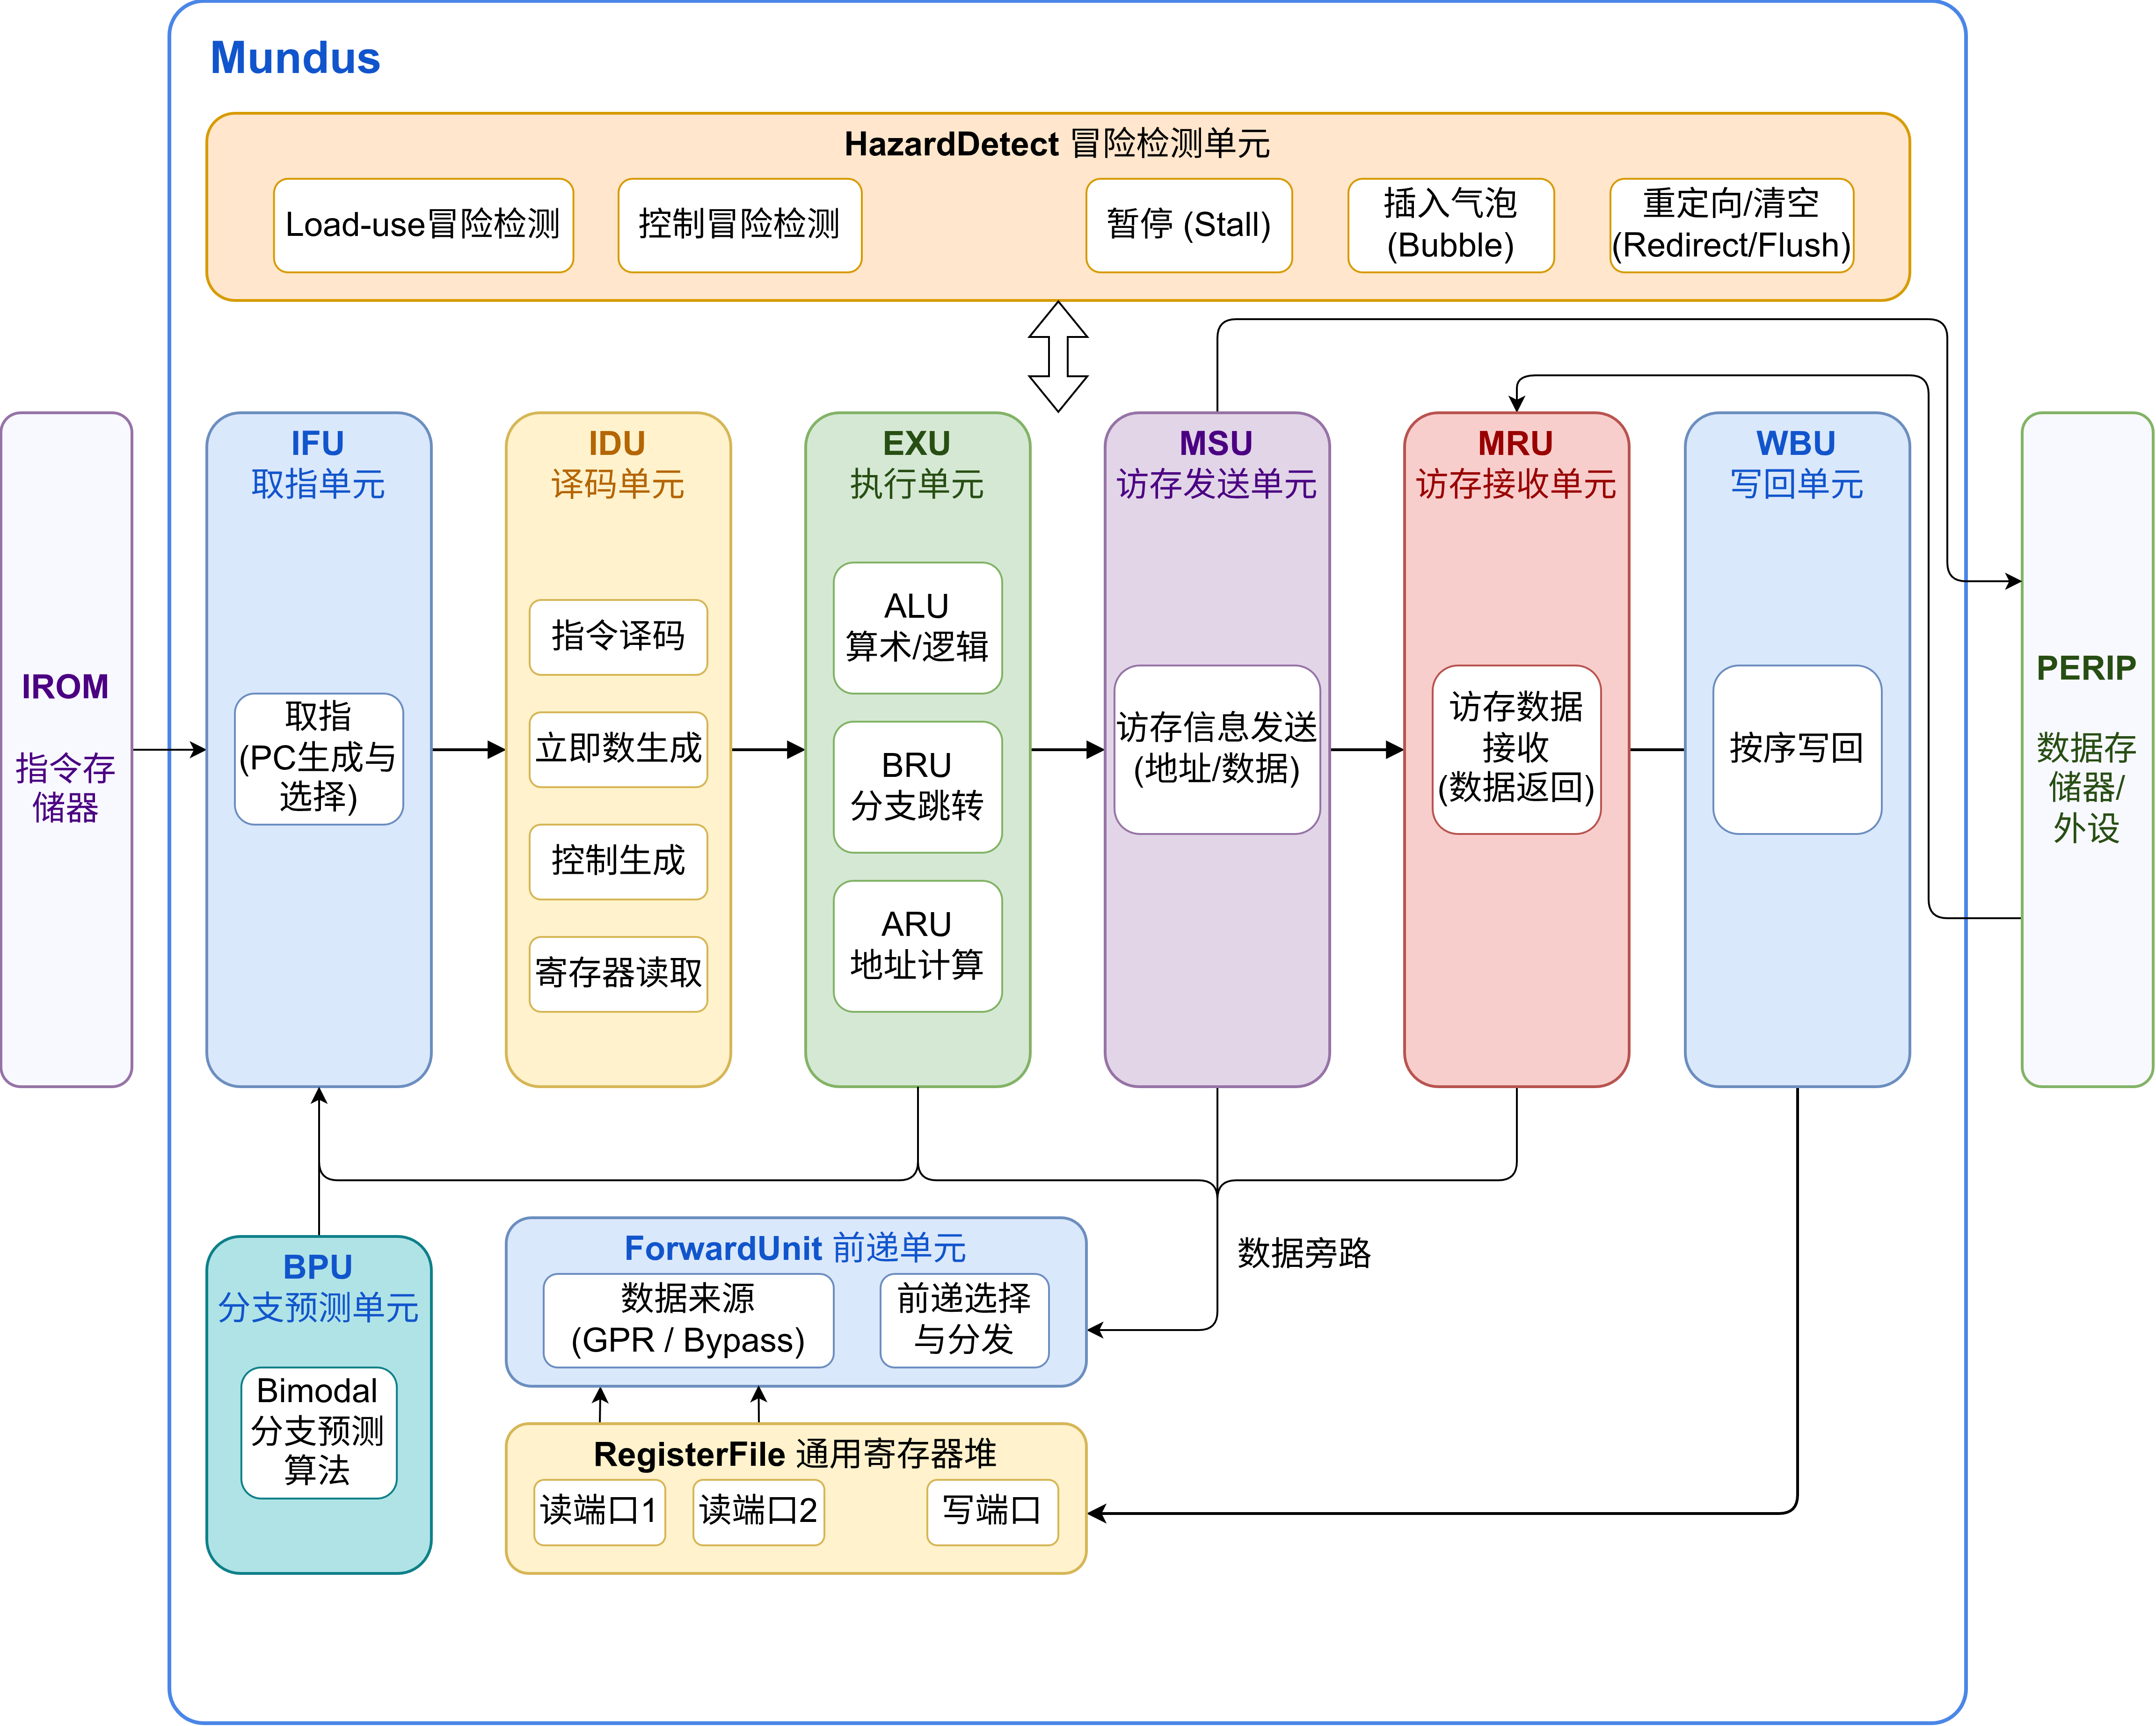
\includegraphics[width=1.0\linewidth]{figures/cpu_arch.png}
  \caption{RV32I CPU整体架构图}
  \label{fig:cpu-arch}
\end{figure}


\subsection{数据通路各模块的设计}

本处理器采用六级流水线结构，整体数据通路划分为 IFU、IDU、EXU、LS1、LS2 和 WBU 六个主要阶段，各流水级之间通过流水线寄存器传递数据。流水线控制单元根据数据冒险、控制冒险和访存状态产生 stall、bubble 和 flush 信号，用于控制各级流水寄存器是否保持、清空或正常更新。

从整体执行流程看，IFU 负责根据 PC 从 IROM 取出指令，并结合分支预测结果产生下一条取指地址；IDU 负责对指令进行译码，生成立即数和控制信号；EXU 负责完成算术逻辑运算、分支判断和访存地址计算；LS1 负责向数据存储器或外设接口发起访存请求；LS2 负责接收访存返回数据并完成 load 数据扩展；WBU 负责将最终结果写回通用寄存器堆。通过这种流水划分方式，处理器能够在多个时钟周期中并行处理多条指令，从而提高指令吞吐率。

\subsubsection{PC与IFU（取指）模块}

IFU（Instruction Fetch Unit）是处理器流水线的第一级，主要负责维护当前取指地址 PC，并根据 PC 从指令存储器 IROM 中取出 32 bit 指令。IFU 的输出包括当前指令的 PC、顺序下一条地址 snpc、取出的指令 inst，以及分支预测模块给出的预测信息。这些信息会被锁存到 IF/ID 流水线寄存器中，供后续译码阶段使用。

PC 的更新需要同时考虑复位、控制冒险重定向、流水线暂停以及分支预测等情况。为了保证处理器在异常控制流和流水线阻塞情况下仍然能够正确执行，本设计中 PC 更新采用固定优先级。其优先级从高到低依次为：

\begin{enumerate}
    \item 当复位信号有效时，PC 被初始化为程序入口地址；
    \item 当执行级检测到分支预测错误或跳转目标错误时，PC 被重定向为 EXU/BRU 给出的真实地址；
    \item 当流水线因数据冒险或访存等待而暂停时，PC 保持当前值不变；
    \item 当 BPU 预测当前指令需要跳转且 BTB 命中时，PC 更新为 BPU 给出的预测目标地址；
    \item 在无跳转、无重定向、无暂停的普通情况下，PC 更新为顺序地址 PC + 4。
\end{enumerate}

本设计中的 IROM 作为指令存储器，为取指阶段提供指令机器码。IFU 每周期根据当前 PC 产生 IROM 地址，并将返回的指令送入 IF/ID 流水寄存器。若流水线未发生 stall 或 flush，则 IF/ID 在时钟上升沿锁存当前取指结果；若发生 stall，则 IF/ID 保持原值；若发生 flush，则 IF/ID 被清空或写入无效指令。通过这种方式，IFU 能够同时支持正常顺序取指、预测跳转取指、流水线暂停以及错误路径冲刷。

\subsubsection{IDU（译码）模块}

从 IF/ID 流水寄存器接收指令，从指令中解析opcode、rd、rs1、rs2 字段，并根据 RV32I 指令格式生成 I、S、B、U、J 五类立即数。

除了以上基本的指令译码结果以外 ，同时还生成了ALU（算术逻辑单元）的操作码、ALU两个源操作数的选择信号、BRU 控制信号、寄存器写使能、访存写使能、访存宽度和加载符号扩展控制信号，方便后续对执行单元进行控制。

完整控制信号表见2.4 数据通路信号表。

\subsubsection{EXU（执行）模块}

EXU 是主要执行阶段，内部包含 ALU、BRU 和 AGU 三个部分。ALU 负责整数算术逻辑运算，BRU 负责分支判断和跳转目标计算，AGU 负责 load/store 指令的访存地址计算。

ALU 支持 RV32I 所需的加法、减法、逻辑与、逻辑或、异或、移位、有符号比较和无符号比较等操作。其输入由 IDU 生成的操作数选择信号决定，可以来自 rs1、rs2、立即数、pc 或 snpc。

\begin{figure}[H]
  \centering
  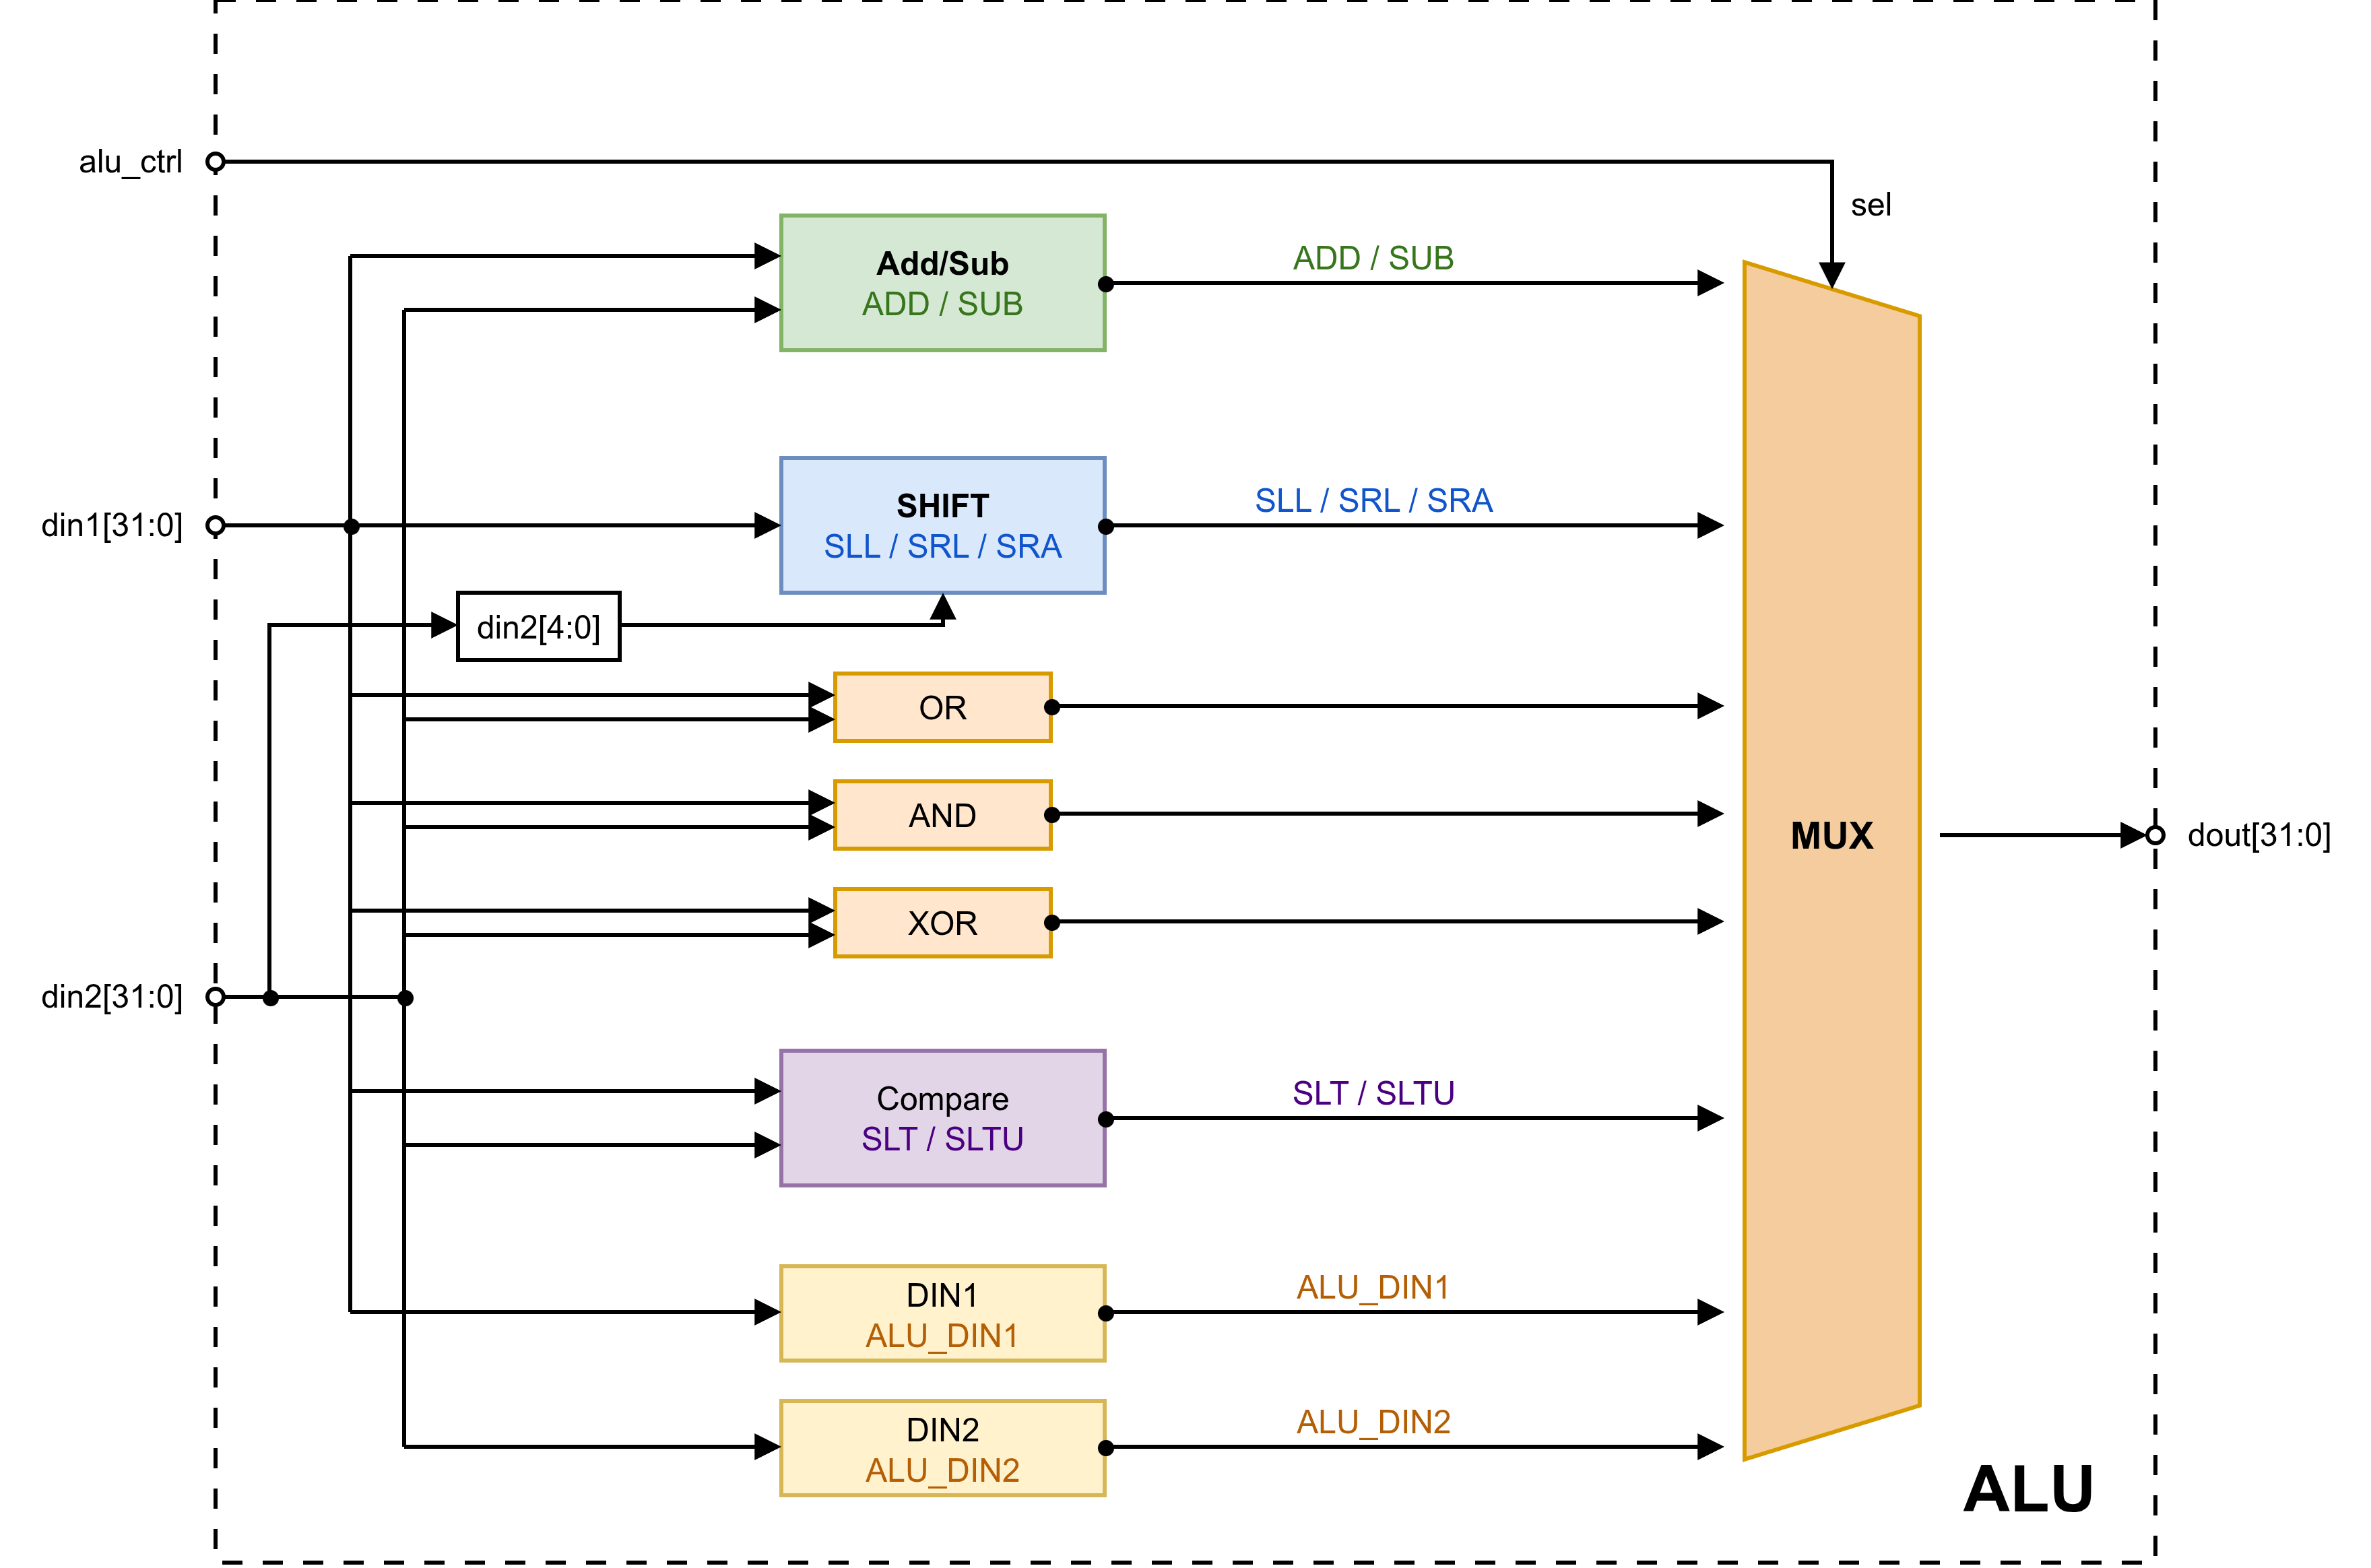
\includegraphics[width=0.90\linewidth]{figures/ALU.png}
  \caption{ALU 模块示意图}
\end{figure}

BRU 负责处理 \code{beq}、\code{bne}、\code{blt}、\code{bge}、\code{bltu}、\code{bgeu}、\code{jal} 和 \code{jalr} 等控制流指令。对于条件分支指令，BRU 根据比较结果决定真实 next\_pc；对于 \code{jal}，真实 next\_pc 为 pc + imm；对于 \code{jalr}，真实 next\_pc 为 (rs1 + imm) \& \textasciitilde{}1。EXU 会将真实 next\_pc 与前端预测地址进行比较，若二者不一致，则触发 flush，并将 PC 重定向到正确地址。

对于 load/store 指令，AGU 计算访存地址 rs1 + imm，并将访存地址、写数据、访存宽度和读写控制信号传递给 LS1。

\subsubsection{LS1 访存请求模块}

LS1 负责发起访存请求。它接收 EXU 计算出的访存地址、store 写数据、访存宽度和读写控制信号，并将这些信息输出到 PERIP 接口。

对于 store 指令，LS1 根据 \code{sb}、\code{sh}、\code{sw} 的类型生成对应写数据和写掩码，分别完成字节、半字和字写入。对于 load 指令，LS1 发出读请求，并将访存地址、访存宽度和符号扩展控制信号继续传递给 LS2。

\subsubsection{LS2 访存返回模块}

LS2 负责接收 PERIP 接口返回的读数据，并根据 load 指令类型进行数据截取和扩展。对于 \code{lb}、\code{lh} 指令，LS2 对读取出的字节或半字进行符号扩展；对于 \code{lbu}、\code{lhu} 指令，LS2 进行零扩展；对于 \code{lw} 指令，LS2 直接使用完整 32 bit 读数据。

对于非 load 指令，LS2 不进行访存数据处理，只将 EXU 或 LS1 传来的执行结果继续向后传递。LS2 的输出包括最终候选写回数据、目的寄存器编号和写回控制信号，这些信息会进入 LS2/WB 流水寄存器，并在 WBU 阶段完成写回。

本设计将传统访存阶段拆分为 LS1 和 LS2 两级，主要是为了适配 FPGA 中 BRAM 的读返回延迟，同时降低单级组合逻辑复杂度，提高流水线可达主频。

\subsubsection{WBU（写回）模块}

WBU以LS2的输出作为输入，并输出目的寄存器地址、写使能和写回数据，并连接到寄存器堆的写端口，为后续写入寄存器做好准备。

\subsubsection{寄存器组与数据转发模块}

RegisterFile（寄存器组）的地址宽度为 5 bit。寄存器堆提供两个读端口和一个写端口，写回阶段在 wbu\_valid 且写使能有效时写入寄存器。本设计的通用寄存器堆（GPR）采用同步读写设计，在Vivado中可被综合为BRAM。同时为了避免同步读带来额外一周期的数据冒险，本设计为了不复杂化旁路网络，没有选择给ForwardUnit增加WBU的旁路，而是选择将GPR输出网络设计为写优先，从而兼顾BRAM的优秀读写时序和简化数据旁路网络

ForwardUnit（数据转发单元）比较 IDU 阶段源寄存器与 EXU/LS1/LS2 阶段目的寄存器，处理数据冒险。由于访存流水被拆成 LS1 和 LS2，当前转发路径也从一般的 EXU/LSU 扩展为 EXU/LS1/LS2。

\subsection{数据通路信号表}

\begin{normaltable}
\begin{longtable}{@{}L{0.20\linewidth}L{0.24\linewidth}L{0.52\linewidth}@{}}
\caption{数据通路信号说明表}\label{tab:datapath-signal-desc}\\
\toprule
\textbf{信号名} & \textbf{含义} & \textbf{取值 / 说明} \\
\midrule
\endfirsthead
\toprule
\textbf{信号名} & \textbf{含义} & \textbf{取值 / 说明} \\
\midrule
\endhead
\bottomrule
\endfoot
\code{inst_type} & 立即数类型 & R / I / S / B / U / J \\
\code{ALU_operand1} & ALU 源操作数 1 选择 & 选择 ALU 第一个输入操作数 \\
\code{ALU_operand2} & ALU 源操作数 2 选择 & 选择 ALU 第二个输入操作数 \\
\code{ALU_ctrl} & ALU 运算控制 & 指定 ALU 执行的运算类型 \\
\code{bru_ctrl} & 分支/跳转控制 & 控制条件分支与跳转指令 \\
\code{rd_wen} & 寄存器写回使能 & \code{REG_WRITE} 表示写回寄存器 \\
\code{mem_wen} & 存储器访问方向 & \code{MEM_WRITE} 表示写存储器；\code{MEM_READ} 表示读存储器 / 非写 \\
\code{mem_bytes} & 访存宽度 & \code{MEM_BYTE} / \code{MEM_HALF} / \code{MEM_WORD} / \code{MEM_NONE} \\
\code{L_sign} & load 指令扩展方式 & \code{SIGNED} / \code{UNSIGNED} \\
\code{snpc} & 顺序下一条指令地址 & 通常表示 PC + 4，用于顺序取指、跳转链接写回等场景 \\
\code{pc} & 当前指令地址 & 用于取指、\code{auipc} 计算与分支跳转目标计算 \\
\code{shamt} & 移位立即数 & 用于 \code{slli}、\code{srli}、\code{srai} 等立即数移位指令 \\
\code{wbu_valid} & 写回阶段有效标记 & 与写使能共同决定是否写入通用寄存器 \\
\code{load} & load类型指令标记 & 用于LS2选择内存读数据或EXU运算结果作为写回数据 \\
\code{PERIP} & 数据存储器/外设接口 & 用于访存请求发送与读数据返回 \\
\code{IROM} & 指令存储器接口 & 根据PC地址返回32 bit指令 \\
\end{longtable}
\end{normaltable}

\begin{tighttable}
\begin{longtable}{@{}L{0.07\linewidth}C{0.05\linewidth}L{0.11\linewidth}L{0.20\linewidth}L{0.15\linewidth}L{0.29\linewidth}L{0.10\linewidth}@{}}
\caption{RV32I各指令数据通路信号表}\label{tab:datapath-instructions}\\
\toprule
\textbf{指令} & \textbf{Imm} & \textbf{Reg读} & \textbf{ALU / 写回通路} & \textbf{LSU / 访存通路} & \textbf{BRU / PC 通路} & \textbf{Reg写} \\
\midrule
\endfirsthead
\toprule
\textbf{指令} & \textbf{Imm} & \textbf{Reg读} & \textbf{ALU / AGU / 写回通路} & \textbf{LSU / 访存通路} & \textbf{BRU / PC 通路} & \textbf{Reg写} \\
\midrule
\endhead
\bottomrule
\endfoot
\code{add} & 无 & rs1, rs2 & rs1 + rs2 & 无 & pc $\leftarrow$ snpc & rd $\leftarrow$ ALU 结果 \\
\code{sub} & 无 & rs1, rs2 & rs1 - rs2 & 无 & pc $\leftarrow$ snpc & rd $\leftarrow$ ALU 结果 \\
\code{addi} & I & rs1 & rs1 + imm & 无 & pc $\leftarrow$ snpc & rd $\leftarrow$ ALU 结果 \\
\code{lui} & U & 无 & 直通 imm & 无 & pc $\leftarrow$ snpc & rd $\leftarrow$ imm \\
\code{auipc} & U & 无 & imm + pc & 无 & pc $\leftarrow$ snpc & rd $\leftarrow$ ALU 结果 \\
\code{and} & 无 & rs1, rs2 & rs1 \& rs2 & 无 & pc $\leftarrow$ snpc & rd $\leftarrow$ ALU 结果 \\
\code{or} & 无 & rs1, rs2 & rs1 \textbar{} rs2 & 无 & pc $\leftarrow$ snpc & rd $\leftarrow$ ALU 结果 \\
\code{xor} & 无 & rs1, rs2 & rs1 $\wedge$ rs2 & 无 & pc $\leftarrow$ snpc & rd $\leftarrow$ ALU 结果 \\
\code{andi} & I & rs1 & rs1 \& imm & 无 & pc $\leftarrow$ snpc & rd $\leftarrow$ ALU 结果 \\
\code{ori} & I & rs1 & rs1 \textbar{} imm & 无 & pc $\leftarrow$ snpc & rd $\leftarrow$ ALU 结果 \\
\code{xori} & I & rs1 & rs1 $\wedge$ imm & 无 & pc $\leftarrow$ snpc & rd $\leftarrow$ ALU 结果 \\
\code{slt} & 无 & rs1, rs2 & 有符号比较：rs1 $<$ rs2 & 无 & pc $\leftarrow$ snpc & rd $\leftarrow$ 比较结果 \\
\code{sltu} & 无 & rs1, rs2 & 无符号比较：rs1 $<$ rs2 & 无 & pc $\leftarrow$ snpc & rd $\leftarrow$ 比较结果 \\
\code{slti} & I & rs1 & 有符号比较：rs1 $<$ imm & 无 & pc $\leftarrow$ snpc & rd $\leftarrow$ 比较结果 \\
\code{sltiu} & I & rs1 & 无符号比较：rs1 $<$ imm & 无 & pc $\leftarrow$ snpc & rd $\leftarrow$ 比较结果 \\
\code{sll} & 无 & rs1, rs2 & rs1 $\ll$ rs2[4:0] & 无 & pc $\leftarrow$ snpc & rd $\leftarrow$ ALU 结果 \\
\code{srl} & 无 & rs1, rs2 & rs1 $\gg$ rs2[4:0]，逻辑右移 & 无 & pc $\leftarrow$ snpc & rd $\leftarrow$ ALU 结果 \\
\code{sra} & 无 & rs1, rs2 & rs1 \texttt{>>>} rs2[4:0]，算术右移 & 无 & pc $\leftarrow$ snpc & rd $\leftarrow$ ALU 结果 \\
\code{slli} & I & rs1 & rs1 $\ll$ shamt & 无 & pc $\leftarrow$ snpc & rd $\leftarrow$ ALU 结果 \\
\code{srli} & I & rs1 & rs1 $\gg$ shamt，逻辑右移 & 无 & pc $\leftarrow$ snpc & rd $\leftarrow$ ALU 结果 \\
\code{srai} & I & rs1 & rs1 \texttt{>>>} shamt，算术右移 & 无 & pc $\leftarrow$ snpc & rd $\leftarrow$ ALU 结果 \\
\code{lb} & I & rs1 & 计算访存地址：rs1 + imm & 读 1 字节，符号扩展 & pc $\leftarrow$ snpc & rd $\leftarrow$ sext(mem[7:0]) \\
\code{lh} & I & rs1 & 计算访存地址：rs1 + imm & 读 2 字节，符号扩展 & pc $\leftarrow$ snpc & rd $\leftarrow$ sext(mem[15:0]) \\
\code{lw} & I & rs1 & 计算访存地址：rs1 + imm & 读 4 字节 & pc $\leftarrow$ snpc & rd $\leftarrow$ mem[31:0] \\
\code{lbu} & I & rs1 & 计算访存地址：rs1 + imm & 读 1 字节，零扩展 & pc $\leftarrow$ snpc & rd $\leftarrow$ zext(mem[7:0]) \\
\code{lhu} & I & rs1 & 计算访存地址：rs1 + imm & 读 2 字节，零扩展 & pc $\leftarrow$ snpc & rd $\leftarrow$ zext(mem[15:0]) \\
\code{sb} & S & rs1, rs2 & 计算访存地址：rs1 + imm & 写入 rs2[7:0] & pc $\leftarrow$ snpc & 无 \\
\code{sh} & S & rs1, rs2 & 计算访存地址：rs1 + imm & 写入 rs2[15:0] & pc $\leftarrow$ snpc & 无 \\
\code{sw} & S & rs1, rs2 & 计算访存地址：rs1 + imm & 写入 rs2[31:0] & pc $\leftarrow$ snpc & 无 \\
\code{beq} & B & rs1, rs2 & 比较操作，无写回 & 无 & 若 rs1 == rs2，pc $\leftarrow$ pc + imm；否则 pc $\leftarrow$ snpc & 无 \\
\code{bne} & B & rs1, rs2 & 比较操作，无写回 & 无 & 若 rs1 != rs2，pc $\leftarrow$ pc + imm；否则 pc $\leftarrow$ snpc & 无 \\
\code{blt} & B & rs1, rs2 & 有符号比较，无写回 & 无 & 若有符号 rs1 $<$ rs2，pc $\leftarrow$ pc + imm；否则 pc $\leftarrow$ snpc & 无 \\
\code{bltu} & B & rs1, rs2 & 无符号比较，无写回 & 无 & 若无符号 rs1 $<$ rs2，pc $\leftarrow$ pc + imm；否则 pc $\leftarrow$ snpc & 无 \\
\code{bge} & B & rs1, rs2 & 有符号比较，无写回 & 无 & 若有符号 rs1 $>=$ rs2，pc $\leftarrow$ pc + imm；否则 pc $\leftarrow$ snpc & 无 \\
\code{bgeu} & B & rs1, rs2 & 无符号比较，无写回 & 无 & 若无符号 rs1 $>=$ rs2，pc $\leftarrow$ pc + imm；否则 pc $\leftarrow$ snpc & 无 \\
\code{jal} & J & 无 & 直通 snpc & 无 & pc $\leftarrow$ pc + imm & rd $\leftarrow$ snpc \\
\code{jalr} & I & rs1 & 直通 snpc & 无 & pc $\leftarrow$ (rs1 + imm) \& \textasciitilde{}1 & rd $\leftarrow$ snpc \\
\end{longtable}
\end{tighttable}

\subsection{控制器设计}

\subsubsection{控制信号表}

\begin{normaltable}
\begin{longtable}{@{}L{0.20\linewidth}C{0.12\linewidth}L{0.64\linewidth}@{}}
\caption{控制信号说明表}\label{tab:control-signal-desc}\\
\toprule
\textbf{控制信号} & \textbf{位宽} & \textbf{核心含义} \\
\midrule
\endfirsthead
\toprule
\textbf{控制信号} & \textbf{位宽} & \textbf{核心含义} \\
\midrule
\endhead
\bottomrule
\endfoot
\code{alu_ctrl} & 12 & ALU 运算操作码 \\
\code{bru_ctrl} & 9 & 分支 / 跳转类型控制 \\
\code{rd_wen} & 1 & 通用寄存器写使能 \\
\code{mem_wen} & 1 & 存储器写使能 \\
\code{mem_bytes} & 2 & 访存宽度 \\
\code{L_sign} & 1 & Load 符号扩展 \\
\code{jump} & 1 & \code{jal}/\code{jalr} 无条件跳转标记 \\
\end{longtable}
\end{normaltable}


\begin{tighttable}
\begin{longtable}{@{}L{0.11\linewidth}L{0.20\linewidth}C{0.12\linewidth}C{0.13\linewidth}C{0.15\linewidth}C{0.12\linewidth}C{0.12\linewidth}@{}}
\caption{运算类、访存类指令控制信号表}\label{tab:control-alu-memory}\\
\toprule
\textbf{指令} & \textbf{alu\_ctrl} & \textbf{rd\_wen} & \textbf{mem\_wen} & \textbf{mem\_bytes} & \textbf{L\_sign} & \textbf{jump} \\
\midrule
\endfirsthead
\toprule
\textbf{指令} & \textbf{alu\_ctrl} & \textbf{rd\_wen} & \textbf{mem\_wen} & \textbf{mem\_bytes} & \textbf{L\_sign} & \textbf{jump} \\
\midrule
\endhead
\bottomrule
\endfoot
\code{add} & \code{12'h4} & 1 & 0 & 3 & 0 & 0 \\
\code{sub} & \code{12'h8} & 1 & 0 & 3 & 0 & 0 \\
\code{addi} & \code{12'h4} & 1 & 0 & 3 & 0 & 0 \\
\code{lui} & \code{12'h2} & 1 & 0 & 3 & 0 & 0 \\
\code{auipc} & \code{12'h4} & 1 & 0 & 3 & 0 & 0 \\
\code{and} & \code{12'h40} & 1 & 0 & 3 & 0 & 0 \\
\code{or} & \code{12'h20} & 1 & 0 & 3 & 0 & 0 \\
\code{xor} & \code{12'h10} & 1 & 0 & 3 & 0 & 0 \\
\code{andi} & \code{12'h40} & 1 & 0 & 3 & 0 & 0 \\
\code{ori} & \code{12'h20} & 1 & 0 & 3 & 0 & 0 \\
\code{xori} & \code{12'h10} & 1 & 0 & 3 & 0 & 0 \\
\code{slt} & \code{12'h400} & 1 & 0 & 3 & 0 & 0 \\
\code{sltu} & \code{12'h800} & 1 & 0 & 3 & 0 & 0 \\
\code{slti} & \code{12'h400} & 1 & 0 & 3 & 0 & 0 \\
\code{sltiu} & \code{12'h800} & 1 & 0 & 3 & 0 & 0 \\
\code{sll} & \code{12'h80} & 1 & 0 & 3 & 0 & 0 \\
\code{srl} & \code{12'h100} & 1 & 0 & 3 & 0 & 0 \\
\code{sra} & \code{12'h200} & 1 & 0 & 3 & 0 & 0 \\
\code{slli} & \code{12'h80} & 1 & 0 & 3 & 0 & 0 \\
\code{srli} & \code{12'h100} & 1 & 0 & 3 & 0 & 0 \\
\code{srai} & \code{12'h200} & 1 & 0 & 3 & 0 & 0 \\
\code{lb} & \code{12'h4} & 1 & 0 & 0 & 1 & 0 \\
\code{lh} & \code{12'h4} & 1 & 0 & 1 & 1 & 0 \\
\code{lw} & \code{12'h4} & 1 & 0 & 2 & 1 & 0 \\
\code{lbu} & \code{12'h4} & 1 & 0 & 0 & 0 & 0 \\
\code{lhu} & \code{12'h4} & 1 & 0 & 1 & 0 & 0 \\
\code{sb} & \code{12'h4} & 0 & 1 & 0 & 0 & 0 \\
\code{sh} & \code{12'h4} & 0 & 1 & 1 & 0 & 0 \\
\code{sw} & \code{12'h4} & 0 & 1 & 2 & 0 & 0 \\
\end{longtable}
\end{tighttable}

\begin{tighttable}
\begin{longtable}{@{}L{0.11\linewidth}L{0.20\linewidth}C{0.12\linewidth}C{0.13\linewidth}C{0.15\linewidth}C{0.12\linewidth}C{0.12\linewidth}@{}}
\caption{分支跳转类指令控制信号表}\label{tab:control-branch}\\
\toprule
\textbf{指令} & \textbf{bru\_ctrl} & \textbf{rd\_wen} & \textbf{mem\_wen} & \textbf{mem\_bytes} & \textbf{L\_sign} & \textbf{jump} \\
\midrule
\endfirsthead
\toprule
\textbf{指令} & \textbf{bru\_ctrl} & \textbf{rd\_wen} & \textbf{mem\_wen} & \textbf{mem\_bytes} & \textbf{L\_sign} & \textbf{jump} \\
\midrule
\endhead
\bottomrule
\endfoot
\code{beq} & \code{9'h09} & 0 & 0 & 3 & 0 & 0 \\
\code{bne} & \code{9'h11} & 0 & 0 & 3 & 0 & 0 \\
\code{blt} & \code{9'h21} & 0 & 0 & 3 & 0 & 0 \\
\code{bltu} & \code{9'h81} & 0 & 0 & 3 & 0 & 0 \\
\code{bge} & \code{9'h41} & 0 & 0 & 3 & 0 & 0 \\
\code{bgeu} & \code{9'h101} & 0 & 0 & 3 & 0 & 0 \\
\code{jal} & \code{9'h04} & 1 & 0 & 3 & 0 & 1 \\
\code{jalr} & \code{9'h04} & 1 & 0 & 3 & 0 & 1 \\
\end{longtable}
\end{tighttable}

\subsubsection{控制器设计说明}

结合给定的 RV32I 指令控制信号表，本 CPU 的控制器整体集成在指令译码阶段，依托指令机器码中的操作码、功能码字段完成全指令集的组合逻辑译码工作，根据不同指令的功能需求，统一生成 alu\_ctrl、bru\_ctrl、rd\_wen、mem\_wen、mem\_bytes、L\_sign、jump 等核心控制信号，以此统筹调度流水线各级硬件模块的工作行为，实现算术逻辑运算、分支跳转、存储器访问与寄存器写回的整体协同运作。

控制器针对不同功能指令完成差异化的控制信号编码配置，通过 12 位的 alu\_ctrl 完成 ALU 运算功能的精准选择，为加减运算、逻辑运算、移位操作、大小比较以及访存地址计算分配独立控制编码，让 ALU 能够依据指令需求完成对应运算处理。9 位的 bru\_ctrl 专门服务于分支与跳转指令，依据 \code{beq}、\code{bne}、\code{blt} 等不同条件分支规则完成编码区分，搭配 jump 标志位区分条件分支与 \code{jal}、\code{jalr} 无条件跳转指令，实现分支跳转逻辑的独立控制。

在存储与写回控制逻辑设计上，控制器利用单比特 rd\_wen 信号管控通用寄存器写使能状态，运算类、移位类、加载类以及跳转链接指令需要结果写回寄存器，该信号置为有效，条件分支与存储类指令无需寄存器写入，默认关闭写使能。mem\_wen 作为存储器写控制信号，仅在 \code{sb}、\code{sh}、\code{sw} 等存储指令中生效，其余指令全部屏蔽内存写操作，配合 mem\_bytes 位宽控制信号，区分字节、半字、字三种访存规格，无访存操作的指令统一配置默认参数，保证硬件资源不会产生无效访问行为。

针对加载指令的特殊需求，控制器设置 L\_sign 控制信号专门管理符号扩展逻辑，对 \code{lb}、\code{lh} 等有符号加载指令开启符号扩展，对 \code{lbu}、\code{lhu} 无符号加载指令关闭符号扩展，精准匹配 RV32I 加载指令的内存数据读取规则。整体控制器采用纯组合逻辑译码架构，以指令原始字段作为输入，直接输出稳定的控制信号组合，信号随流水线寄存器逐级传递，同时结合硬件冒险检测机制，在数据冒险与控制冒险场景下配合气泡、暂停机制修正控制信号生效逻辑，保障六级流水线运行过程中的稳定性与正确性，整套控制信号编码规则规整统一，指令与控制参数一一对应，让控制器具备结构简洁、逻辑清晰、易于拓展的设计特点。

\section{流水线功能设计}

本设计采用 IFU、IDU、EXU、LS1、LS2、WBU 六级流水线结构，分别完成取指、译码、执行、访存请求发送、访存数据接收和写回。相较于传统五级流水线，本设计将访存阶段进一步拆分为 LS1 和 LS2 两级，使访存请求发送、访存数据返回和写回处理之间的边界更加清晰，也更适合同步读存储器接口。

顶层 Mundus 中显式实例化了六个流水级模块，并通过 pipelineConnect 在相邻流水级之间传递数据，同时接入 stall 与 bubble 控制信号，以支持流水线暂停和气泡插入。整体流水线结构如图~\ref{fig:Pipeline_Structure}所示。

\begin{figure}[H]
  \centering
  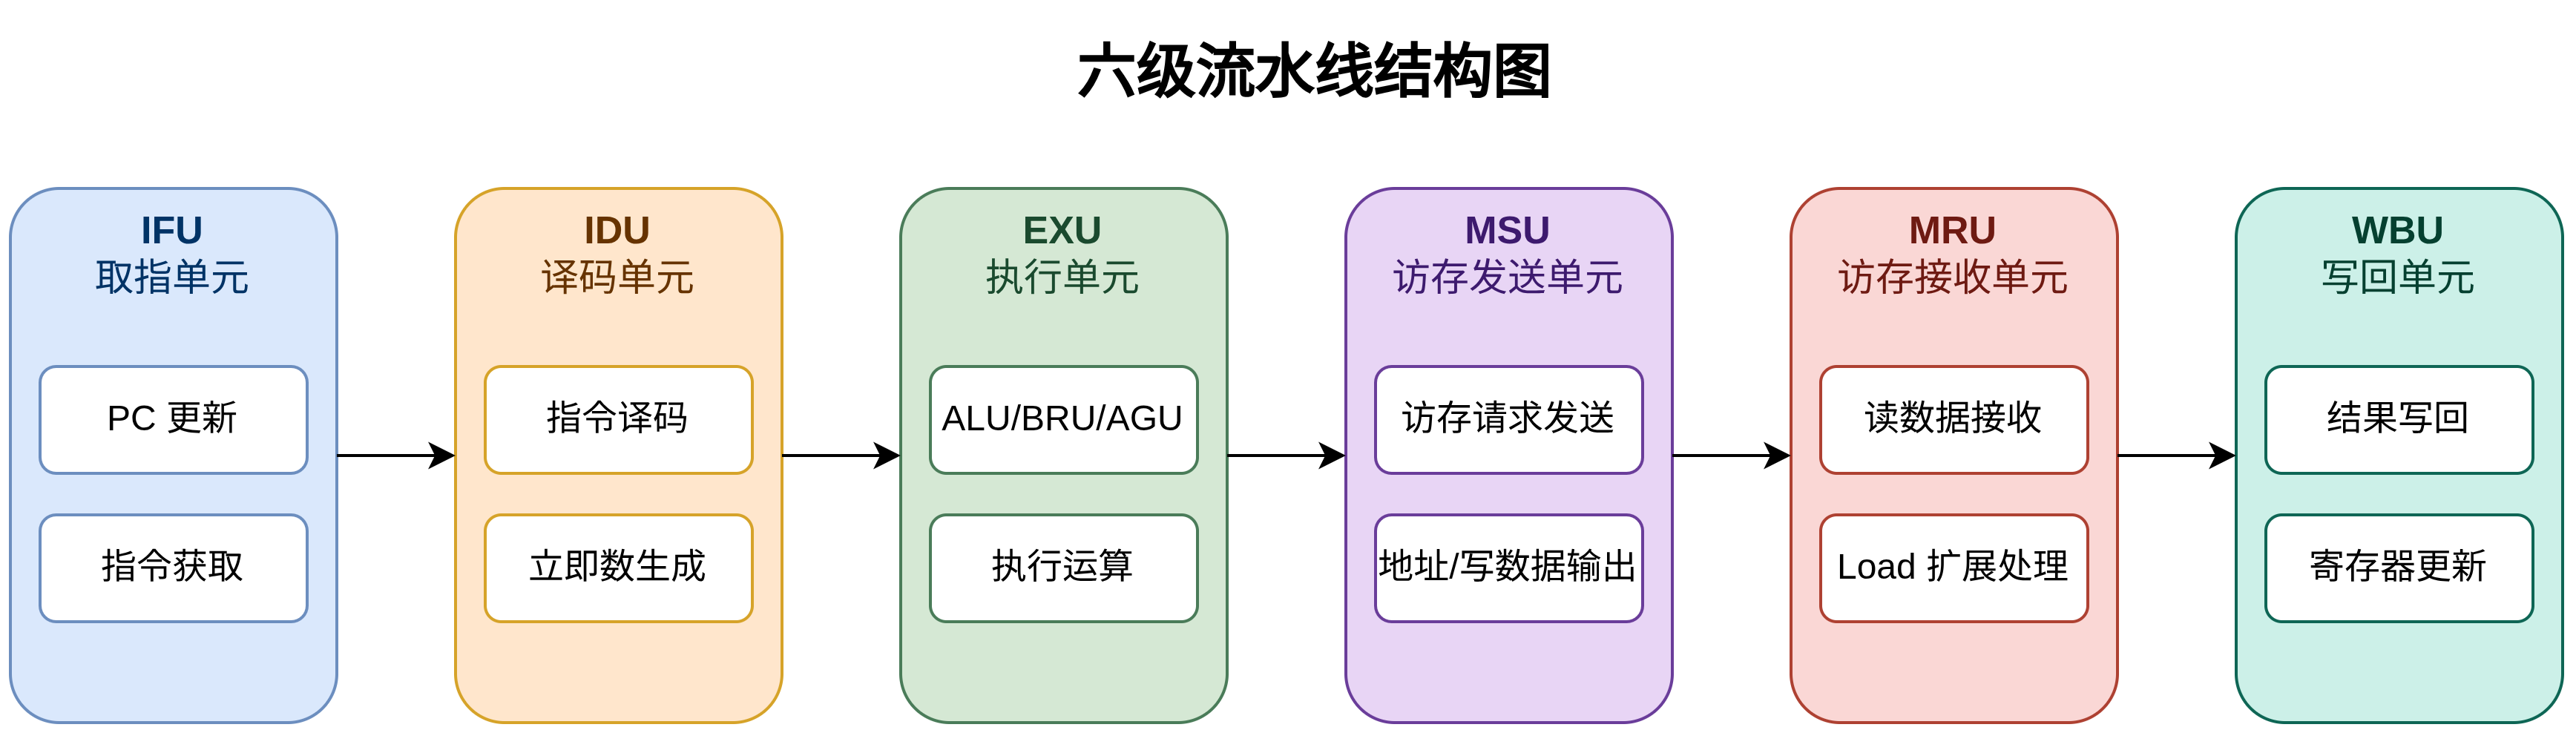
\includegraphics[width=0.90\linewidth]{figures/Pipeline_Structure.png}
  \caption{六级流水线示意图}
  \label{fig:Pipeline_Structure}
\end{figure}

\subsection{六级流水线结构}

六级流水线各阶段的主要功能如下：

\begin{itemize}
  \item \textbf{IFU：}负责根据当前 PC 从 IROM 中取出指令，并结合分支预测结果生成下一条取指地址。
  \item \textbf{IDU：}负责解析指令字段，生成立即数、寄存器编号和后续流水级所需的控制信号。
  \item \textbf{EXU：}负责完成 ALU 运算、分支判断、跳转目标计算和访存地址计算。
  \item \textbf{LS1：}负责向外部存储器或外设接口发送访存地址、写使能、写数据和字节掩码。
  \item \textbf{LS2：}负责接收访存返回数据，并根据 load 指令类型完成数据截取、符号扩展或零扩展。
  \item \textbf{WBU：}负责将最终计算结果或访存结果写回通用寄存器堆。
\end{itemize}

其中，LS1 和 LS2 的拆分是本设计区别于典型五级流水线的重要部分。传统五级流水线通常将访存请求生成、数据返回和 load 数据处理放在同一级中，而本设计将其拆成两个阶段，可以降低单级组合逻辑复杂度，并适配 FPGA 中常见的同步读存储器结构。

\begin{figure}[H]
  \centering
  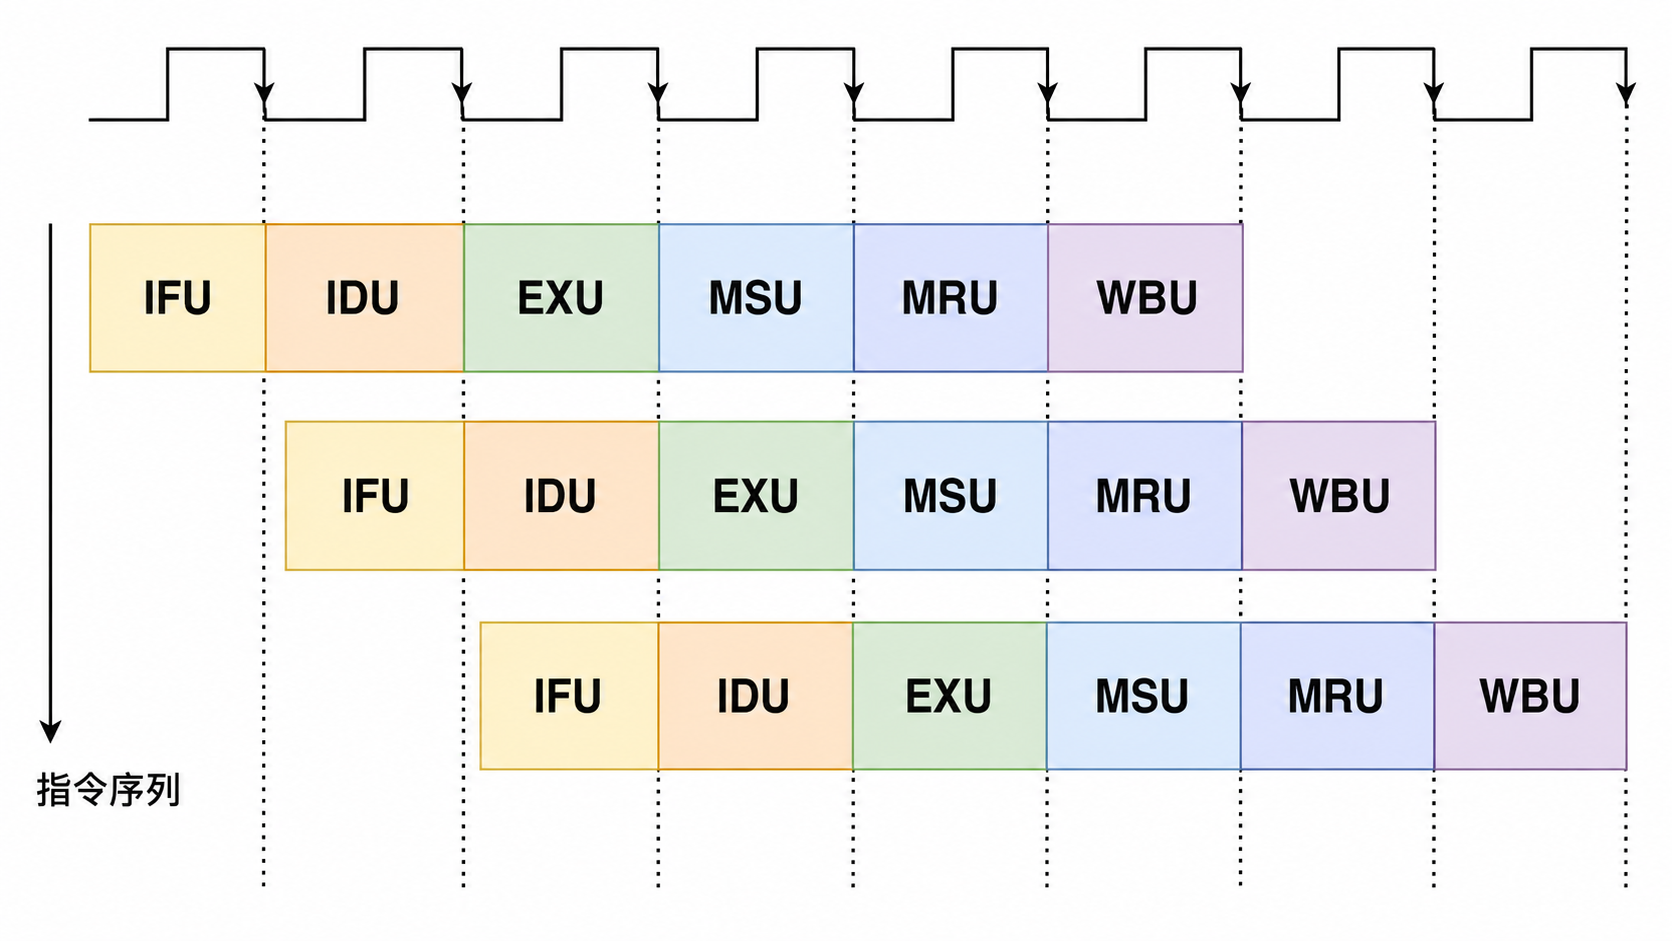
\includegraphics[width=0.90\linewidth]{figures/pipeline.png}
  \caption{六级流水线执行波形图}
\end{figure}

\subsection{流水线数据前递}

为了减少 RAW 数据冒险带来的流水线停顿，本设计实现了面向 EXU 操作数输入的数据前递机制。ForwardUnit 从 EXU、LS1、LS2 三个后续流水级收集可能需要前递的结果，并根据 IDU 阶段给出的源寄存器编号选择最新数据，最终输出 rs1\_val和 rs2\_val 供 EXU 使用。

前递优先级按照流水线距离由近到远排列：EXU 优先，其次 LS1，最后 LS2。当多个后续流水级同时写回同一个目的寄存器时，该优先级可以保证 EXU 获得距离当前指令最近、也就是最新的结果。

该机制可以减少多数 ALU-ALU、ALU-branch、ALU-store 等 RAW 冒险造成的停顿，使后续指令能够尽早使用前序指令的计算结果。对于 load 指令，由于数据要到 LS2 阶段才完成接收与扩展，因此仍然需要通过冒险检测逻辑处理 load-use 场景。

\subsection{冒险信号仲裁}

程序运行中可能同时出现控制冒险和数据冒险。本设计通过 HazardDetect 对不同冒险进行集中仲裁，并采用控制冒险优先于数据冒险的策略。这样设计的原因是：一旦分支预测失败或跳转目标错误，当前流水线中的部分指令已经属于错误路径，此时优先清空错误路径比处理数据相关更加重要。

该仲裁逻辑使流水线控制行为更加确定。控制冒险主要触发 flush 或 bubble，用于清空错误路径指令；数据冒险主要触发 stall 或 bubble，用于暂停前级流水线并插入气泡。各级 stall 和 bubble 信号在顶层统一连接到流水线寄存器控制端，从而形成完整的流水线控制闭环。

典型的 load-use 冒险如下：

\begin{center}
\begin{tabular}{l}
\code{lw}\quad \code{x1}, 0(\code{x2}) \\
\code{add}\quad \code{x3}, \code{x1}, \code{x4}
\end{tabular}
\end{center}

第一条 load 指令需要等到 LS2 阶段才能得到内存读数据，而第二条 \code{add} 指令在 EXU 阶段就需要使用 \code{x1} 的值。因此，当冒险检测单元发现后一条指令依赖前一条 load 指令的目的寄存器时，会暂停前端流水线并插入气泡，直到 load 数据可以通过 LS2 前递给后续指令，或在写回阶段通过写优先寄存器堆被后续指令读取。在本设计中，load-use 冒险需要 2 周期阻塞，如图~\ref{fig:load-use}所示

\begin{figure}[H]
  \centering
  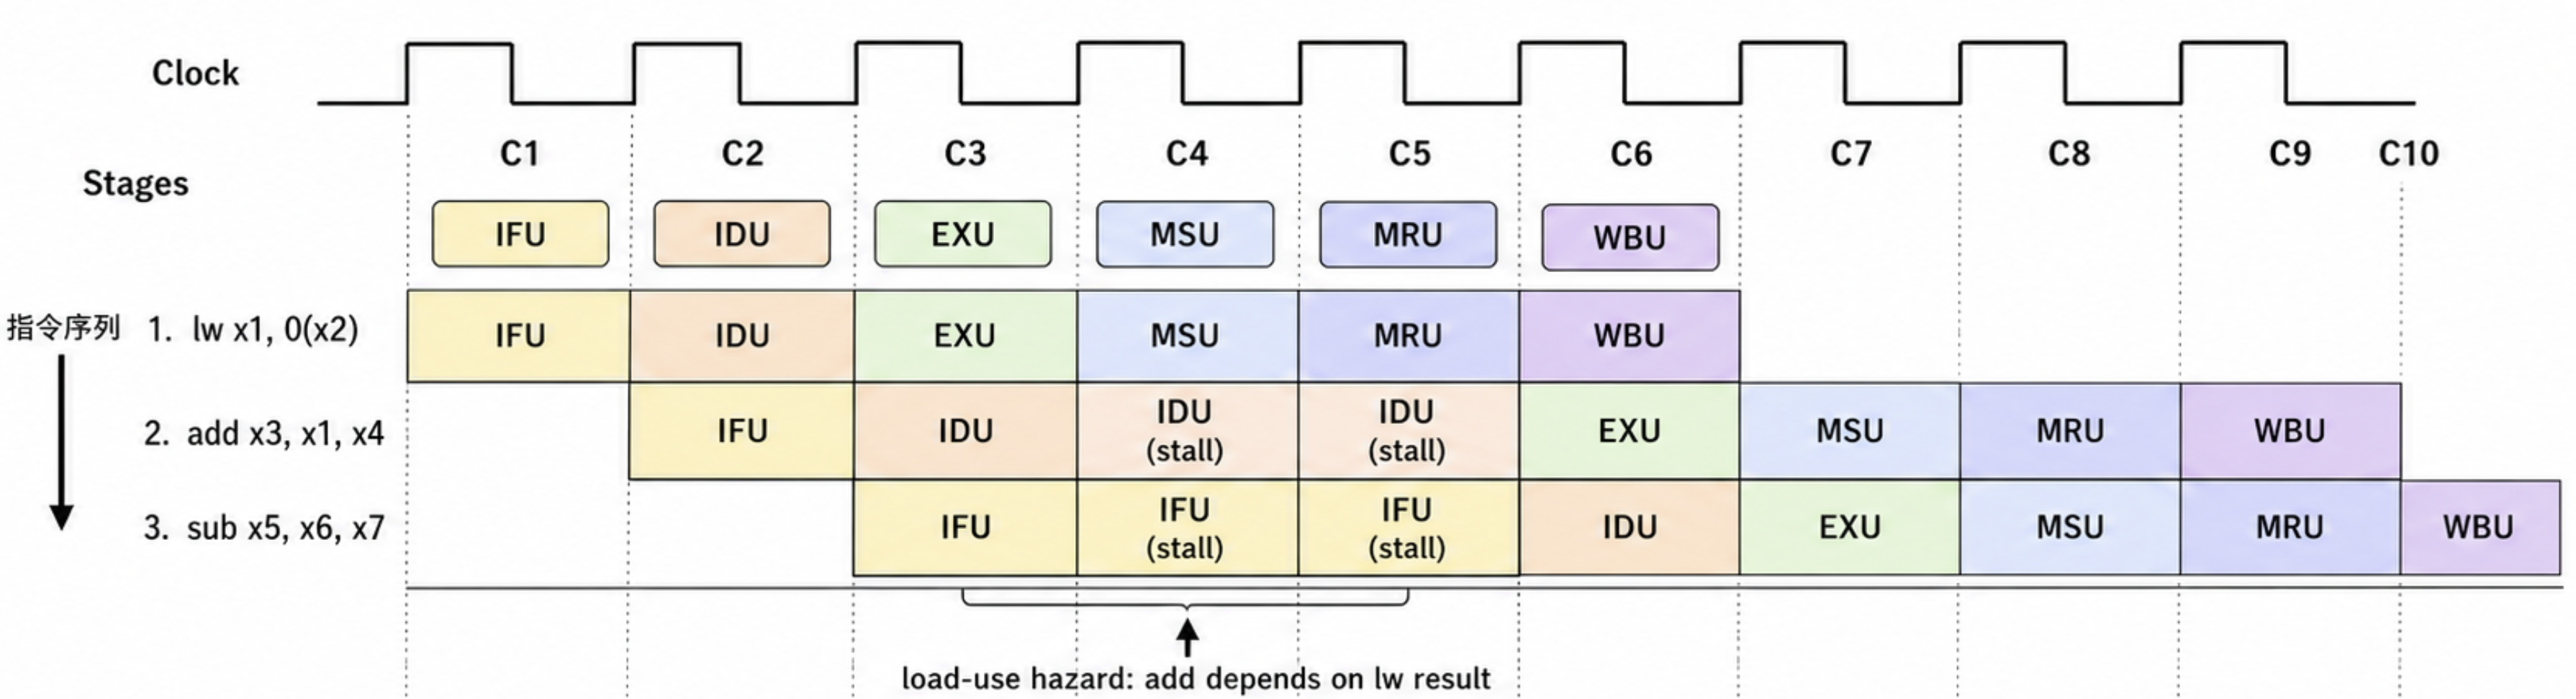
\includegraphics[width=0.90\linewidth]{figures/load-use.png}
  \caption{load-use 冒险波形图}
  \label{fig:load-use}
\end{figure}

\subsection{控制冒险重定向与分支预测}

本设计具备分支预测与分支重定向能力。IFU 中的 BPU 可以根据当前 PC 给出预测方向和预测目标地址；EXU 中的 BRU 负责计算真实跳转结果；当预测 PC 与实际 PC 不一致时，控制冒险单元触发流水线清空和 PC 重定向。

\begin{figure}[H]
  \centering
  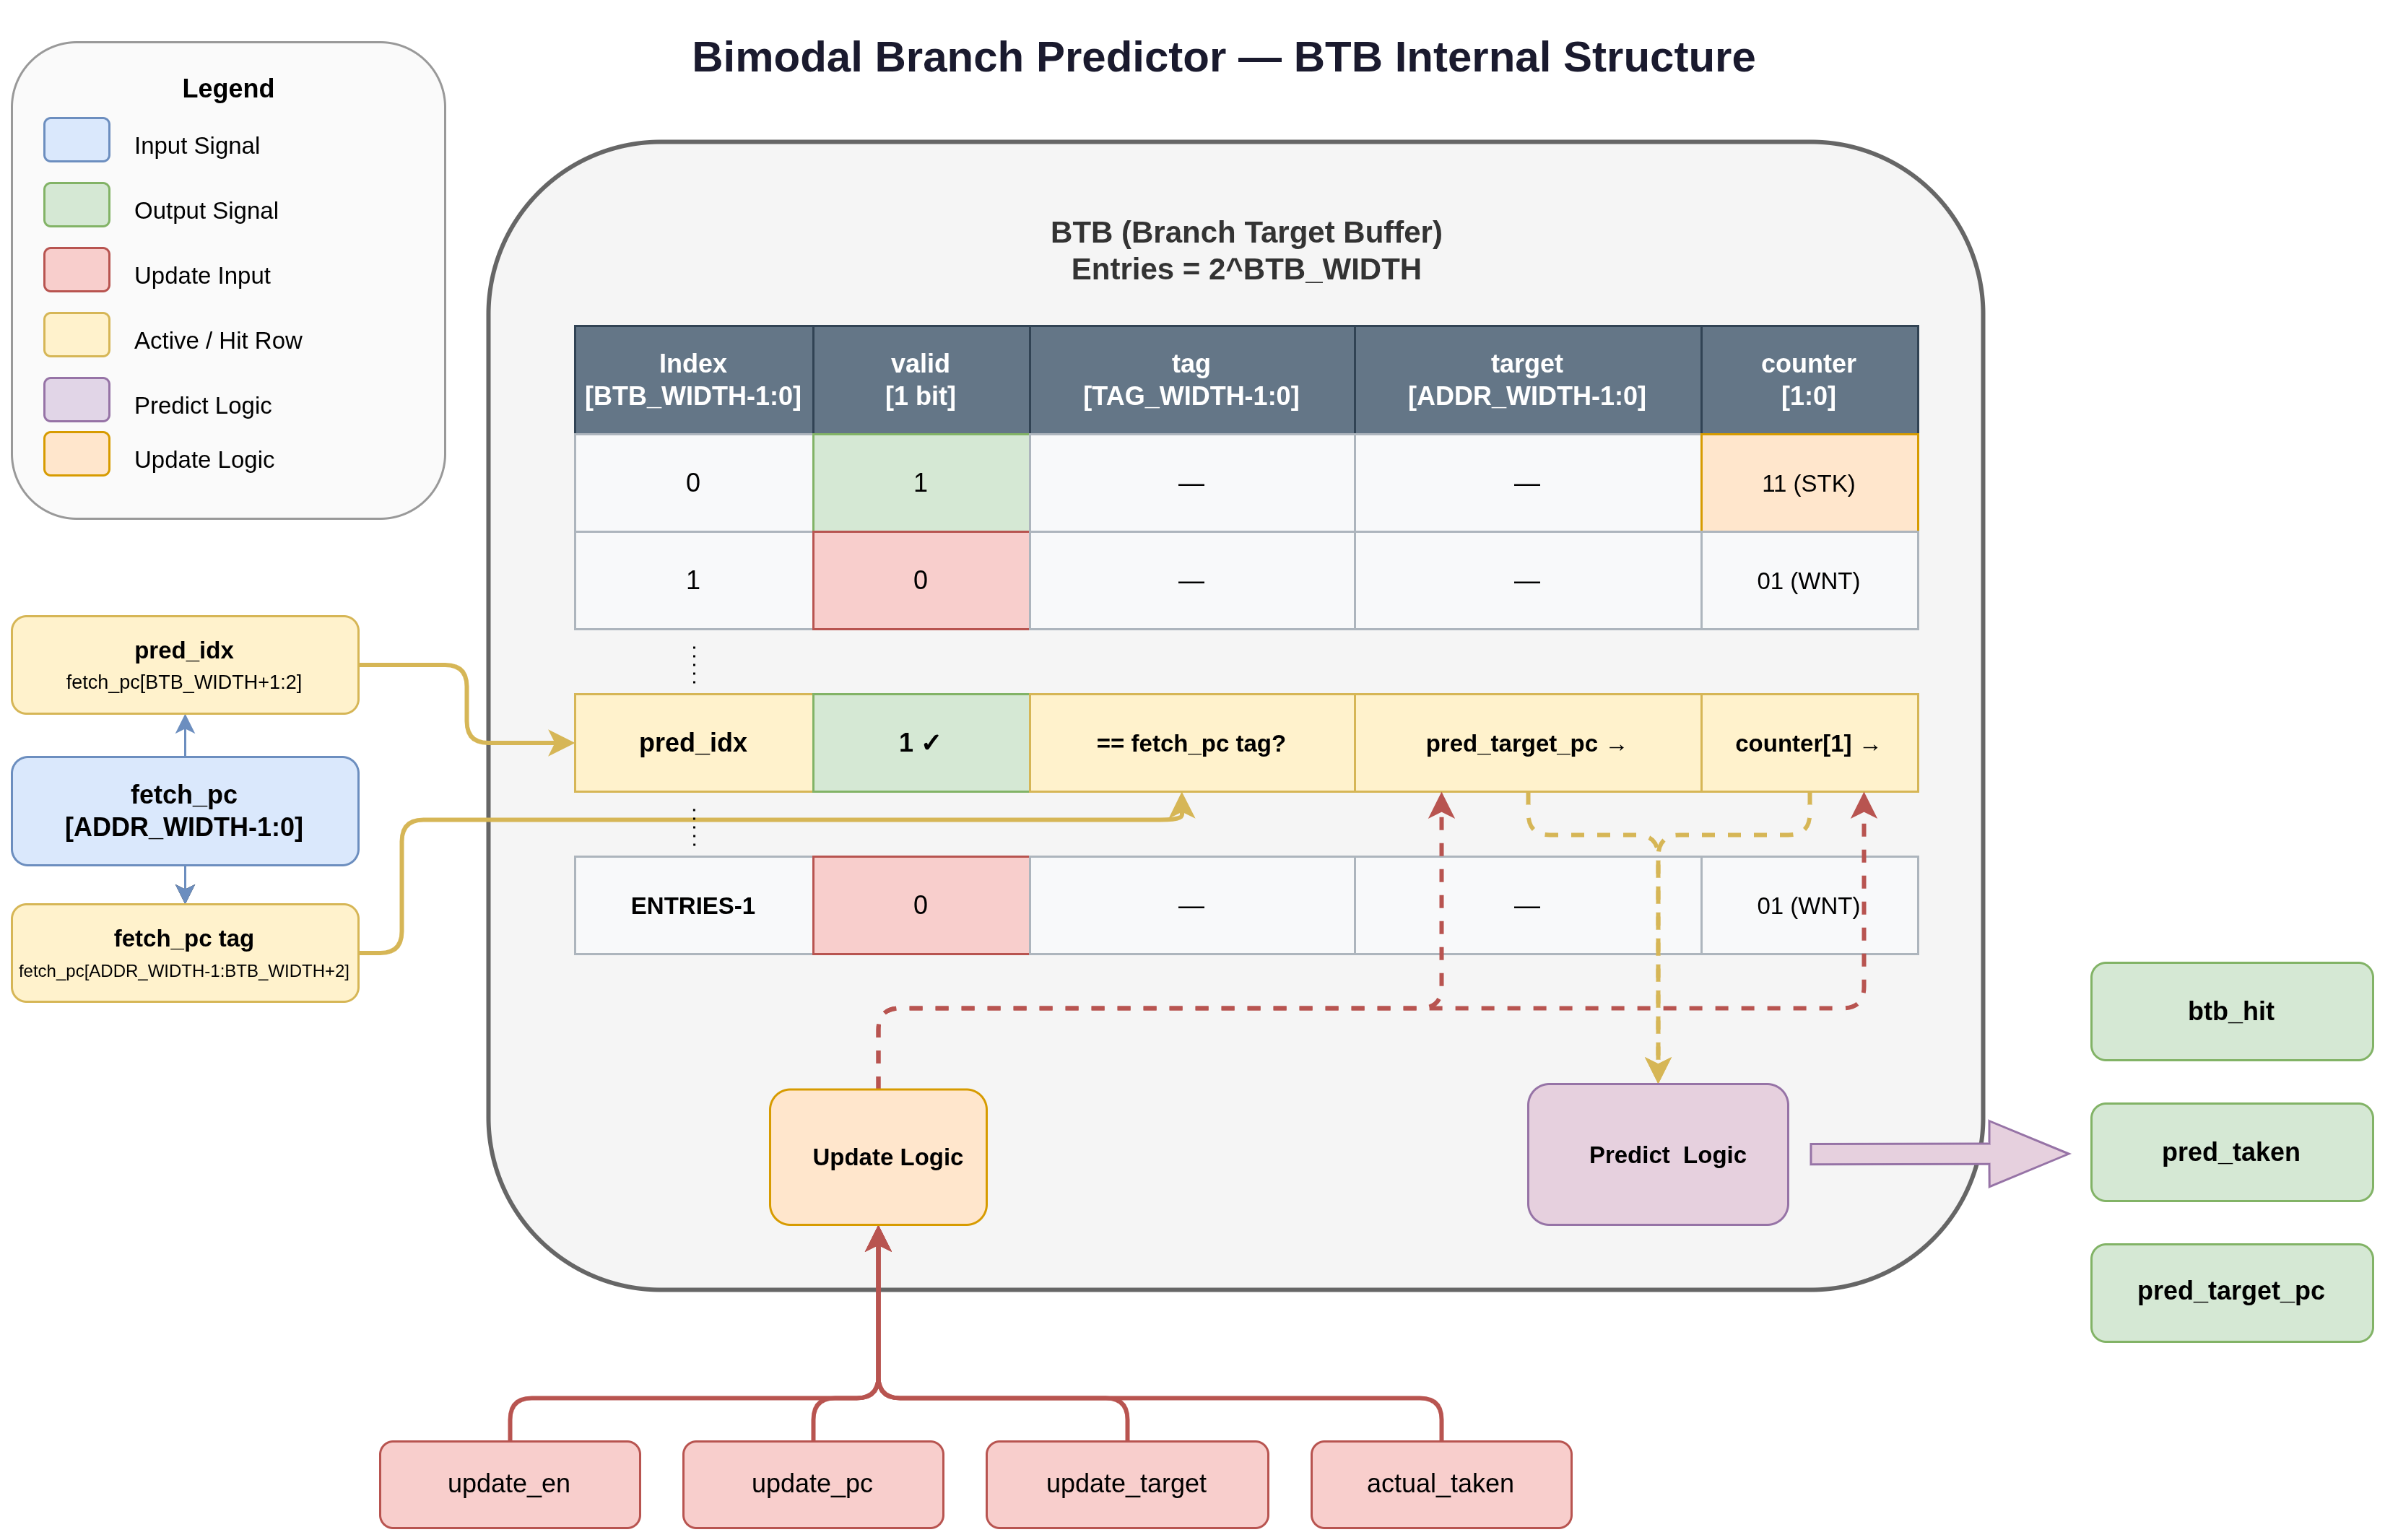
\includegraphics[width=1.0\linewidth]{figures/fi_btb.png}
  \caption{Branch Target Buffer 结构示意图}
\end{figure}

BPU 内部采用 BTB 存储分支指令 PC 及其历史跳转目标地址，为了记录该分支的历史跳转倾向，
我们在每个 BTB 表项中维护一个 2-bit 饱和计数器\cite{smith1981study}，
研究表明 2-bit 计数器在预测准确率与硬件开销之间取得了最优平衡，增加计数器位宽收益甚微。倘若在BTB中没有找到相应的合法记录，则选择不跳转，即预测PC+4作为下一条执行指令。同时，我们在EXU模块执行完毕之后，会输出相应的信号让BTB内部的数据进行相应的更新，以此来学习分支的跳转行为。

本设计在原有 BTB 的基础上实现了 bimodal 分支预测器。当前实现中，PHT（Pattern History Table）并没有作为独立表存在，而是与 BTB 表项一一对应，每个 BTB 表项内部维护一个 2-bit 饱和计数器 counter，用于记录该 PC 历史上是否倾向跳转。

BTB 采用直接映射结构，表项数量由参数 BTB\_WIDTH 决定，在本次 bimodal 测试中取值为8，因此一共有 256 个表项。

索引使用取指 PC 的低位对齐后地址位，由于 RISC-V 指令地址按 4 字节对齐，最低两位 PC[1:0] 不参与索引。剩余高位作为 tag，用于判断 BTB 表项是否命中。

\begin{table}[htbp]
  \centering
  \caption{2-bit 饱和计数器状态定义}
  \begin{normaltable}
  \begin{tabular}{ccc}
    \toprule
    状态名称 & 编码 & 含义 \\
    \midrule
    SNTK & \texttt{2'b00} & Strong Not Taken，强不跳转 \\
    WNTK & \texttt{2'b01} & Weak Not Taken，弱不跳转 \\
    WTK  & \texttt{2'b10} & Weak Taken，弱跳转 \\
    STK  & \texttt{2'b11} & Strong Taken，强跳转 \\
    \bottomrule
  \end{tabular}
  \end{normaltable}
\end{table}

复位后，所有 BTB 表项的 valid 位被清零，同时计数器初始化为 WNTK，即弱不跳转状态。这意味着程序刚开始执行或 BTB 尚未学习到该分支行为时，预测器整体更倾向于预测不跳转。

在引入 bimodal 分支预测器后，预测效果相比 always-not-taken 有明显提升。我们利用Coremark测试程序，总预测准确率从 33.65\% 提升到 70.75\%，分支预测准确率从 37.79\% 提升到 70.26\%。同时，估算的误预测次数由约 151.09M 降低到约 66.60M，减少了约 84.50M 次，说明 bimodal 预测器能够有效学习分支和跳转指令的历史行为，显著提升预测准确性。

\subsubsection{预测逻辑}

预测阶段，BPU 首先使用当前 fetch\_pc 访问 BTB。如果对应表项有效且 tag 匹配，则认为 BTB hit；否则认为 BTB miss。
在 BTB miss 的情况下，预测器不会给出跳转预测，而是默认选择顺序执行。

在 BTB hit 的情况下，预测器读取对应表项中的 2-bit counter，并使用 counter 的最高位作为方向预测依据，
也就是说，当 counter最高位为1 时，预测 taken；当 counter 为最高位为 0 时，预测 not taken。

预测规则可以总结为：

\begin{equation}
  \text{pred\_taken} =
  \begin{cases}
    1, & \text{BTB hit 且 counter[1] = 1} \\
    0, & \text{BTB miss 或 counter[1] = 0}
  \end{cases}
\end{equation}

若预测 taken，则使用 BTB 中保存的历史目标地址 target[pred\_idx] 作为预测跳转目标；若预测 not taken，则前端继续取 PC + 4。

\subsubsection{训练逻辑}

训练阶段发生在 EXU 模块得到真实执行结果之后。EXU 会输出该分支或跳转指令的真实跳转方向 actual\_taken 以及真实目标地址 update\_target，并通过 update\_en 触发 BTB/PHT 更新。
更新时，预测器使用 update\_pc 重新计算索引，将该表项置为有效，写入新的 tag 和真实目标地址。
同时，根据真实跳转结果对 2-bit counter 进行饱和更新。若真实结果为 taken，则 counter 向强跳转方向递增；若真实结果为 not taken，则 counter 向强不跳转方向递减。

该机制能够使预测器逐渐学习循环、条件分支和跳转指令的历史行为。对于稳定跳转的分支，counter 会逐渐进入 WTK/STK 状态；对于稳定不跳转的分支，counter 会逐渐进入 WNTK/SNTK 状态。

如果预测失败，会产生 2 周期的 Miss Penalty

\begin{figure}[H]
  \centering
  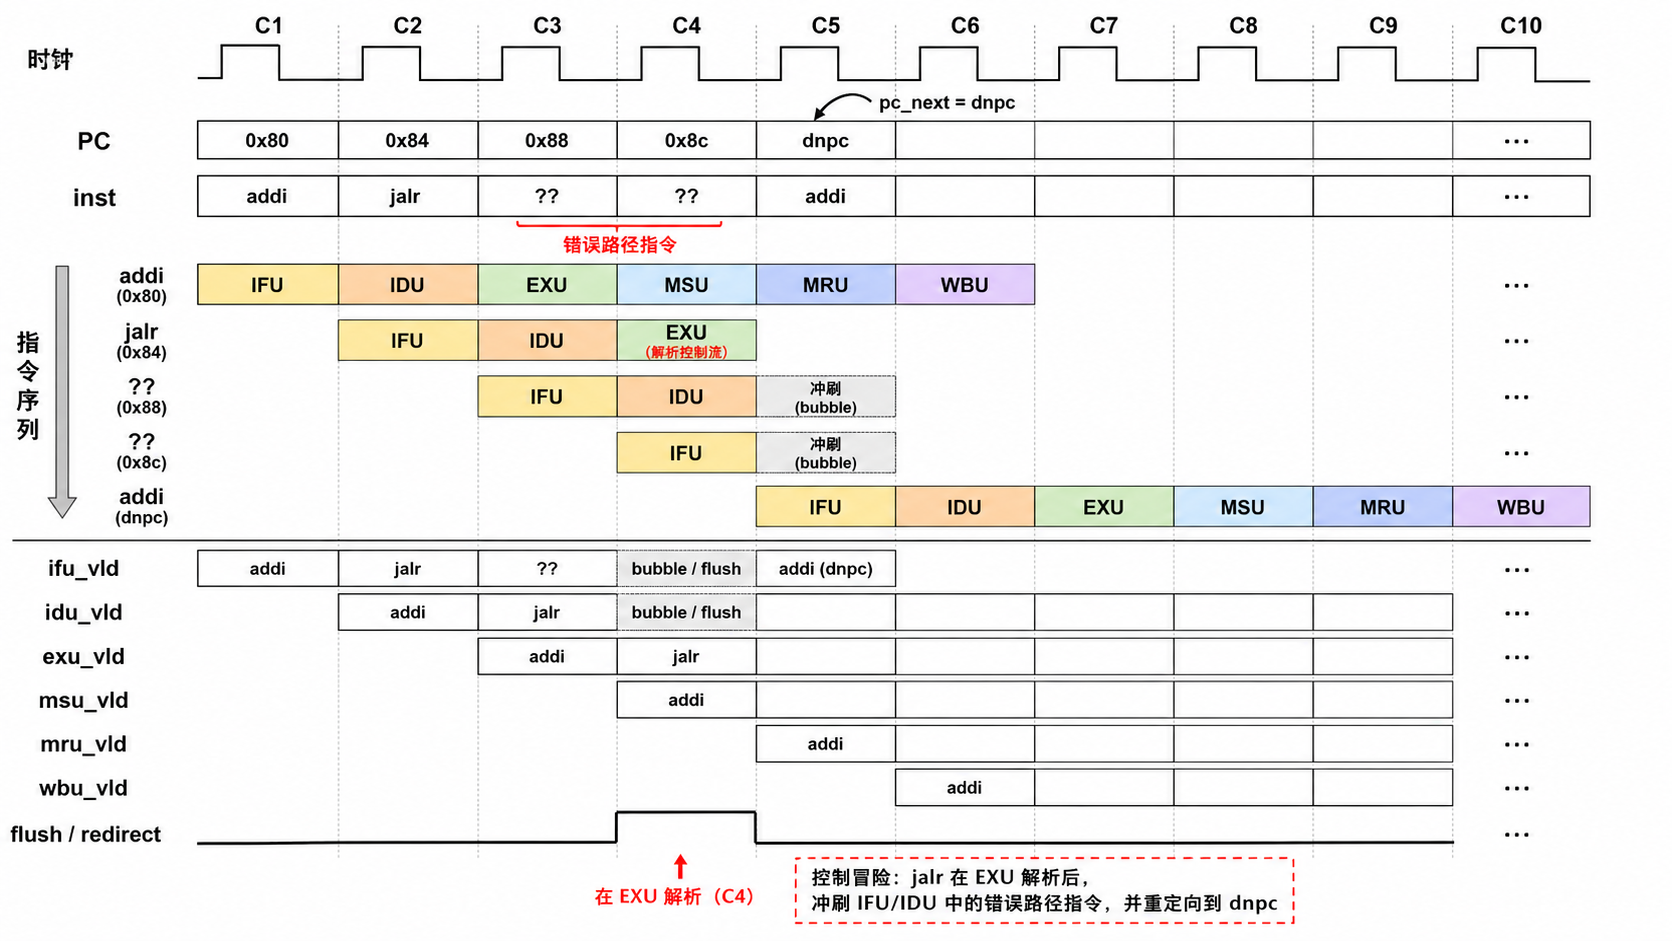
\includegraphics[width=1.0\linewidth]{figures/control-hazard.png}
  \caption{control-hazard 冒险波形图}
\end{figure}

\nocite{smith1995microarchitecture}
\nocite{mittal2019survey}
\renewcommand{\bibname}{参考资料}
\printbibliography

\section{附录}

\subsection{工程目录结构}

\begin{minipage}{\linewidth}
\begin{Verbatim}[fontsize=\small]

// 总体项目目录

Mundus
├── abstract-machine        // 运行时环境
├── am-kernels              // 功能和性能测试程序
├── docs                    // 文档
├── nemu                    // 差分测试 ref
└── npc                     // CPU 核心代码

// 处理器相关核心代码

npc
├── build                   // 仿真环境 Verilator 构建代码
├── configs                 // 配置文件
├── constr                  // Vivado 约束文件
├──csrc                     // C++ 仿真环境代码
│   ├── include             // C++ 头文件
│   └── wave                // 仿真部分核心代码
│       └── utils           // 常用函数或其他工具
├── FormalTest              // 测试验证代码
├── out                     // mill 构建代码
├── scripts                 // tools 文件夹用到的 Makefile script
├── scsrc                   // CPU 核心 Chisel 代码
├── tools                   // 仿真环境用到的开源工具
└── vsrc                    // CPU 核心 Verilog/SystemVerilog 代码
    ├── build               // Chisel 编译出的代码
    ├── include             // Verilog 头文件
    ├── Mundus              // CPU 核心 Verilog/SystemVerilog 代码
    └── testbench           // Verilog 仿真环境
        └── jyd             // perip_bridge 和 IROM 的仿真代码
\end{Verbatim}
\end{minipage}

\subsection{代码清单}

\begin{minipage}{\linewidth}
\begin{Verbatim}[fontsize=\small]

// Chisel核心设计代码

scsrc
├── ALU.scala
├── BPU.scala
├── BRU.scala
├── common.scala                        // 常用 Bundle 和 Scala 函数定义
├── Config.scala                        // 全局手动配置
├── ControlHazard.scala
├── DataHazard.scala
├── EXU.scala
├── ForwardUnit.scala
├── HazardDetect.scala
├── IDU.scala
├── IFU.scala
├── LS1.scala
├── LS2.scala
├── MundusPayloads.scala                // 流水线寄存器数据 Payload
├── Mundus.scala                        // 顶层模块代码
├── MundusSubModules.scala              // Verilog 子模块 Blackbox 定义
└── WBU.scala

\end{Verbatim}
\end{minipage}

\begin{minipage}{\linewidth}
\begin{Verbatim}[fontsize=\small]

// Verilog 核心设计代码

vsrc
├── build
│   └── Mundus.v                        // Chisel 编译的 CPU 核心代码
├── include
│   ├── ALU_flag_para.vh
│   ├── AXI_para.vh
│   ├── common_para.vh
│   ├── device_para.vh
│   ├── inst_para.vh
│   └── SRAM_para.vh
├── Mundus
│   ├── Bimodal.v                       // Bimodal 分支预测器代码
│   ├── HazardDetect_DPIC.v             // 使用 C++ 仿真环境函数的 DPIC 代码
│   ├── IFU_DPIC.v                      // 使用 C++ 仿真环境函数的 DPIC 代码
│   ├── LSU_DPIC.v                      // 使用 C++ 仿真环境函数的 DPIC 代码
│   ├── Mundus_DPIC.v                   // 使用 C++ 仿真环境函数的 DPIC 代码
│   ├── Mundus_PC.v                     // PC 寄存器代码
│   ├── myCPU.v                         // myCPU 模块封装
│   ├── RegisterFile.v                  // 寄存器堆（GPR）
│   └── WBU_DPIC.v                      // 使用 C++ 仿真环境函数的 DPIC 代码
└── testbench
    ├── jyd
    │   ├── bram_driver.sv
    │   ├── BRAM.v                      // BRAM IP Core 的时序仿真代码
    │   ├── cdc_xpm_nofifo_lib.sv       // 解决同步读 perip 的跨时钟域问题
    │   ├── counter.sv
    │   ├── display_seg.sv
    │   ├── dram_driver.sv
    │   ├── DRAM.v                      // DRAM IP Core 的时序仿真代码
    │   ├── IROM.v                      // IROM IP Core 的时序仿真代码
    │   ├── perip_bridge.sv
    │   ├── seg7.sv
    │   └── xpm_cdc_verilator_stubs.sv  // Vivado xpm 模块的 Verilator 封装
    └── MundusJyd.v                     // 仿真环境顶层模块（即 student_top 模块）

\end{Verbatim}
\end{minipage}

\begin{minipage}{\linewidth}
\begin{Verbatim}[fontsize=\small]

// 仿真相关核心代码

csrc
├── include
└── wave
    ├── branch_difftest.cpp             // 分支预测差分测试代码
    ├── cpu.c
    ├── dut.c                           // CPU 功能差分测试代码
    ├── expr.c                          // 表达式求和函数
    ├── main.cpp
    ├── mem.cpp
    ├── reg.cpp
    ├── sdb.c                           // 仿真状态控制函数
    ├── sim.cpp                         // 仿真信息输出函数
    ├── state.c
    ├── trace.c                         // 仿真环境数据 trace
    ├── utils
    │   ├── disasm.c                    // 反汇编工具
    │   └── log.c                       // 日志函数
    └── verilator_ctrl.cpp              // verilator 函数调用
\end{Verbatim}
\end{minipage}

\end{document}
